\documentclass[oneside,final,a4paper]{report}

\usepackage{graphicx}
\usepackage{enumerate}
\usepackage[parfill]{parskip}
\usepackage[section] {placeins}

\graphicspath{{images/}}

\oddsidemargin 0in
\evensidemargin 0in
\textwidth 6.5in 

\begin{document}

% ================ Front Matter ================
% Suppress page number for title page and letter of submittal
\pagestyle{empty}

% ==== Title Page
\begin{flushright}
 \begin{LARGE}
  \textbf{UNIVERSITY OF WATERLOO}
 \end{LARGE}

 \begin{large}
  Faculaty of Mechatronics Engineering\\[4cm]
 \end{large}

 \begin{LARGE}
  \textbf{
    Design Project - Wheelchair Collision Avoidance \\[0.0cm]
    Final Design Report
  }
 \end{LARGE}

 \vfill

  Prepared By: \\[0.2cm]
  Iain Peet - 20252201\\
  Jordan Valentin - 20271260\\
  Rowan Head-Marsden - 20271527\\
  \today
\end{flushright}
\clearpage

% ==== Letter of Transmittal
\today \\[0.5cm]

Faculty of Mechatronics Engineering \\
University of Waterloo \\
Waterloo, Ontario \\

To Whom It May Concern:

This report, entitled \emph{Design Project - Wheelchair Collision Avoidance}, is being prepared for the MTE 481 project by Group 2 and and describes the design of a powered wheel chair collision avoidance system.  The powered wheel chair collision avoidance system that is being designed as a fourth year project by students within the Mechatronics engineering program is designed to provide a affordable solution for the disabled or impaired who are not able to use a wheel chair due to perceived dangers to themselves or others.

We would like to thank Professor Amir Khajepour from the mechanical engineering department who has loaned us a powered wheel chair and provided us with space to work on our project.  

This report was written for the MTE 481 project by the members of group 2 and has not received previous academic credit. \\[0.5cm]

Sincerely, \\[1cm]

Rowan Head-Marsden \hspace {1.5cm} Iain Peet \hspace{1.5cm} Jordan Valentin
\clearpage

% Resume page numbering
\pagestyle{plain}
\setcounter{page}{1}
\pagenumbering{roman}

% ==== Table of Contents
\setcounter{tocdepth}{1}
\tableofcontents

% ==== List of Figures
\listoffigures
\addcontentsline{toc}{chapter}{List of Tables and Figures}

\chapter*{Executive Summary}
\addcontentsline{toc}{chapter}{Summary}
The proposed collision avoidance system for a powered wheel chair is designed to be used by people who are in elder care facilities and would be placed in wheel chairs however there is some concern for their own safety. This means that if the system could guarantee the safety of the user it would be useful and enhance the lives of these people. 

Based on the objectives we have a set of constraints were imposed upon the problem mandating that this must improve the safety of wheel chairs. A set of criteria were laid out to evaluate the designs that had been developed, using measures from the perspective of Costs, Mechanical Capabilities, and Sensing Capabilities. Based on this we evaluated a set of sensors and decided that the Kinect sensor from Microsoft and an array of sonar sensors would be optimal.

Once this was complete we developed a model of the wheel chair and came up with multiple mountings that would suit the needs described earlier in the report. From these, a discussion of each ones benefits and drawbacks was considered. A final design decision was reached regarding the mechanical design and an airplane table tray design was decided to be the final solution moving forward.

 A detailed design section then describes how well the desired mechanical design suits the average human being. Analysis is performed to determine the best orientation of sensors for the purposes of figuring out the range and capabilities of the sonar sensors in those orientations. 

There is a discussion of how the Kinect will work and what the Kinect is along with how it could later be replaced with another system to avoid patent infringement. A discussion of possible tools for the software is also listed including a description of why ROS (robot Operating System) was used for the project.

A schedule has been designed in order to meet the presentation deadline for the completion of the project by March 4th in order to allow time for the preparation of the demo on March 19th. Also a budget of approximately \$750 was laid out for the prototype with an expectation that the final cost will be somewhat lower. 

Based on our observations and our work in progress a set of recommendations were laid for moving forward including the introduction of new wider beam angle ultrasonic sensors, Solutions for dealing with the motor controller, and interface design suggestions.


% ====================== Report Body =================================
\clearpage
\setcounter{page}{1}
\pagenumbering{arabic}
\pagestyle{headings}

\chapter{Introduction}

\section{Background}
Powered wheelchairs have obvious benefits for the mobility of the physically disabled.  Operation of any relatively heavy powered vehicle carries safety risk.  Operators must be capable of safe operation.

Irene Ruel, a physiotherapist in the employ of the British Columbia Interior Health Authority, who has previously been responsible for powered wheelchair assessments in an extended care facilities, was consulted regarding this problem.  By her account, the risk that powered wheelchair operators will collide with other patients is a serious concern.  This risk frequently results in the denial of requests for powered wheelchairs.

\section{Need Statement}
Access to powered wheelchairs may be restricted due to concerns regarding a patient's capability for safe operation.

\section{Objectives and Constraints}
The objectives of this design problem are as follows:

\begin{itemize}
 \item \emph{Improve safety}.  Safety is a significant concern for powered wheelchair operation.  Effective safety systems will be of great value to those with physical disabilities.
 \item \emph{Improve accessibility}.  For those who would be denied access to a powered wheelchair, a safety system which permits access will have significant quality-of-life benefits.
 \item \emph{Assist with difficult tasks}. Some tasks, such as precise positioning and movement in constrained spaces, are difficult even for unimpaired operators.   A system which can assist with such tasks would be helpful.
\end{itemize}

The constraints of this design are as follows:

\begin{itemize}
 \item \emph{Insensitive to operating environment}.  Realistic operating environments will be varied, and subject to change.  The usefulness of a safety system will be severely degraded if it depends on a specialized, controlled environment.
 \item \emph{Integrates with existing wheelchairs}.  Powered wheelchairs are expensive, and many are already in existence.  The potential reach of a new safety system will be severely restricted if it may not be integrated with pre-existing wheelchairs.
 \item \emph{Cost kept below \$500}.  The system will be paid for by end users, who will be sensitive to cost.  It will be difficult to market a system which is very expensive relative to the cost of a basic powered wheelchair.
\end{itemize}

\section{Criteria}
\begin{figure}[hbt]
 \centering
 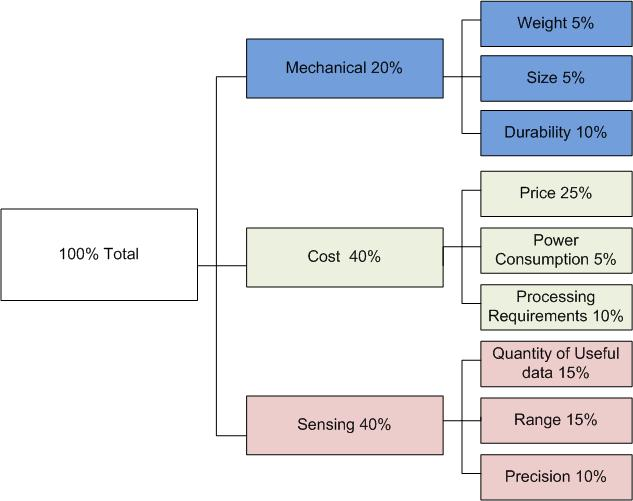
\includegraphics[scale=0.5]{CriteriaWeighting}
 \caption{Criteria Weighting} \label{fig:criteria_weighting}
\end{figure}

\subsection{Weight}
Weight is an important criterion as a number of powered wheel chairs have weight limitations. This should be as small as possible since the weight capacity of a chair like the Invacare Neutron R51LXP is 300 pounds \cite{wheelchair_data}. This means that for any weight we add on to the wheel chair we reduce the potential carrying load of the wheel chair and with it our potential market.

\subsection{Size}
Size is a minor criterion we considered, with an excessively large bulky attachment it would reduce the mobility of the wheel chair and decrease the number of places the wheel chair can travel to. It may also get in the way of the user when operating the wheel chair. This made it important to have some size criteria for measuring the strength of a design.

\subsection{Durability}
While most of the system should not be placed under continuous strain or be at high risk of damage, it is important to consider how durable the design is as there will be wear and tear from use of this system on a wheel chair and damage occurred from movement around the wheel chair.

\subsection{Price}
Price is an important factor for our consideration since we plan to market it to the end users and not to corporations that may have larger budgets. This then made it the most important ranking and with the very large difference in sensor costs it made for a very important factor in determining which route to take.

\subsection{Power Consumption}
Power Consumption measure how much an addition will add to the power consumption of the wheel chair. Many of these chairs are run off of an onboard battery and draining this battery quickly will significantly reduce its usefulness to the users. 

\subsection{Processing Requirements}
The amount of computational intelligence required to handle the data that is coming in from the sensor. This is to make distinction between sensors similar to a Kinect which uses USB and would be plugged into a lab top that will be needed to interpret the data versus something like a sonar sensor that could be tuned and used on FPGA. This will run opposite the Quantity of Useful Data.

\subsection{Quantity of useful Data}
This was selected to distinguish things like sonar which provide simply a distance mapping for a cone versus something like LIDAR, which provides a high-resolution, narrow-beam distance scan. The more data we get from a sensor the more we can make use of it to recognize and avoid obstacles. This runs as the opposite of processing requirements, since more data requires more processing power to interpret the data.

\subsection{Range}
The range for the detection of objects is fairly important to us. While range beyond 7-8 meters is not particularly useful, we want range from about 0 to 8 meters optimally. For this we assume they are working in optimal conditions which we said to be indoors and with normal lighting. Certain sensors we consider have significantly reduced range in other conditions.

\subsection{Precision}
Precision is fairly important since we are detecting obstacles and we would like to know how far away they are, noise and disturbances are acceptable to a small degree so long as we can identify them as noise and not a fast moving obstacle. In addition to this it’s important that some sensors have decreased precision at increased range. This is noted as a small reduction in their score.

\section{Patents}
\subsection{Existing Similar Patents}

\subsubsection{Computer Controlled Power Wheelchair Navigation System}
\begin{figure}[hbt]
 \centering
 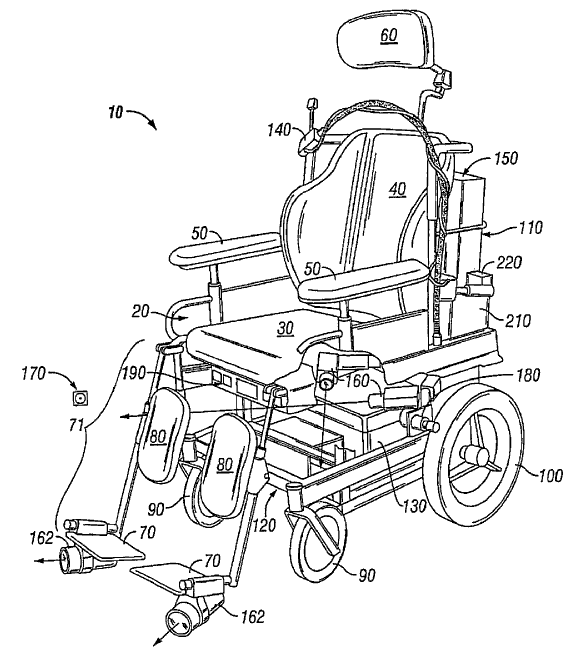
\includegraphics[scale=0.25]{patents}
 \caption{Similar patent \#1 \cite{patent:computer_controlled}}
\end{figure}

The first patent (full patent number, author, and other details listed in \cite{patent:computer_controlled}), entitled \emph{Computer Controlled Power Wheelchair Navigation System}, discusses a patent for wheelchair collision avoidance using cameras, proximity sensors, and microphones.

The chair moves through a marked location and "learns" paths within a home. This makes it less flexible (it cannot operate in unknown environments), and it is unclear how well it works for dynamic obstacles such as people (the objective of our design is to avoid collisions in general, especially with other human beings. Secondly, this device is voice-activated and moves in an automated fashion to the commanded area.

By automating the chair, the user loses the sense of control given by being able to control its movements as wished using a joystick. This is another key difference between this patented design and the goals of this project.

\subsubsection{Powered Wheelchair}
\begin{figure}[hbt]
 \centering
 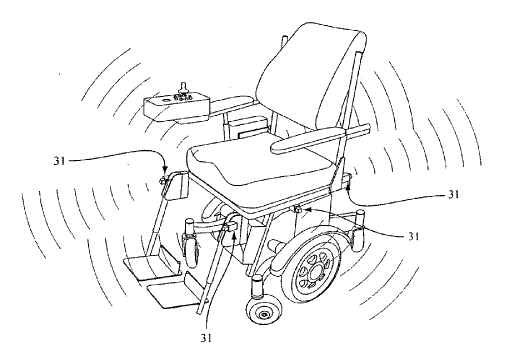
\includegraphics[scale=0.4]{patents2}
 \caption{Similar patent \#2 \cite{patent:power_wheelchair}}
\end{figure}

The second patent (full patent number, author, and other details listed in \cite{patent:power_wheelchair}), entitled \emph{Powered Wheelchair}, discusses a patent for a powered wheelchair with very general collision avoidance specifications.

The patent discusses a "obstacle-detecting sensor" that results in the blocking of a particular input to the chair.

While our design is similar we do not intend to physically block the user from moving the joystick in the direction of travel of a collision. Also, this patent appears to be so general that is fails to discuss any method of sensing or the methods by which obstacles and detected and then blocked. The goals of this design project are very specific in comparison, and do not use any sensors or methods mentioned in this patent. Thus our design is unlikely to infringe on this patent.

\subsubsection{Wheelchair and Method for Correcting the Guidance of a Wheelchair}
\begin{figure}[hbt]
 \centering
 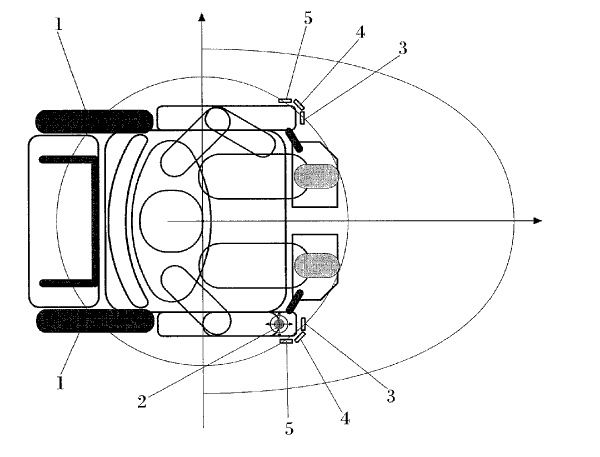
\includegraphics[scale=0.4]{patents3}
 \caption{Similar patent \#3 \cite{patent:wheelchair_method}}
\end{figure}

The third patent (full patent number, author, and other details listed in \cite{patent:wheelchair_method}), entitled \emph{Wheelchair and Method for Correcting the Guidance of a Wheelchair}, discusses a patent for wheelchair collision avoidance system.

It works with two arrays of ultrasound sensors, and decomponses the user commands into forward/backwards linear components and angular components resulting from left/right commands. It determines what space is free in front of the wheelchair and attempts to plan a path.

This patent is similar to our design in that it allows the user control over the wheelchair in terms of motion commands. It is different in its specific implementation, the fact it tries to plan a path through free space rather than rely totally on user input and simply deny movement in unsafe directions, and also in its choice of sensors for collision avoidance.

\subsection{Patentability of this Design}
As shown in the previous section, the design in this report does not appear to infringe on existing patents. That said, many of the sensors and techniques used to implement collision avoidance are not unique and are commonly used in the robotics field for this purpose. It is the specific application of our design to helping the disabled in wheelchairs and the implementation method that are unique. This would limit the patenability of our design since there is no obvious new or novel compoent, and thus the authors will not be a pursuing a patent for this design.

\chapter{Proposed Solution}

\section{Sensor Selection}

Using the criteria mentioned earlier in the report along with their respective weightings, a decision-making matrix was formed and is shown in Table \ref{tab:decision_matrix}.

\begin{figure}[hbt]
 \centering
 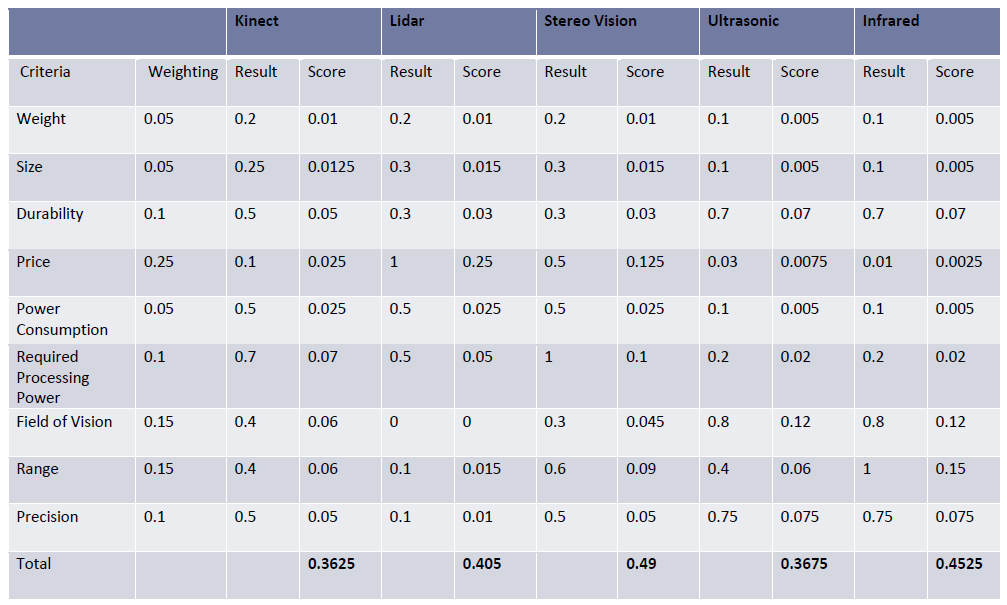
\includegraphics[scale=0.45]{decision_matrix}\\
 \caption{Decision Making Matrix}
 \label{tab:decision_matrix}
\end{figure}

The decision making matrix shows the best sensors according to the projects criteria and weightings, as seen in Table \ref{tab:decision_matrix}. The lowest value was the best in this case since for a number of the criteria lower values represented a better performance such as cost, weight, size, power consumption. This means that the best two sensors were the Xbox Kinect and Sonar. 

These sensors are close in weighting, but operate very differently in practice. The Kinect gives a very large amount of data, both range and bearing, about its field of view. The sonar sensors give less information but are quite cheap. The final solution, since these sensors are weighted so closely, was to use a combination of the two sensors. The Kinect provides accurate and resonably precision data in the direction of movement of the chair, and the sonar sensors provide more coarse collision data about the periphery to prevent collisions from the side.

\section{Mechanical Designs}
\subsection{Design \#1}
\begin{figure}[hbt]
 \centering
 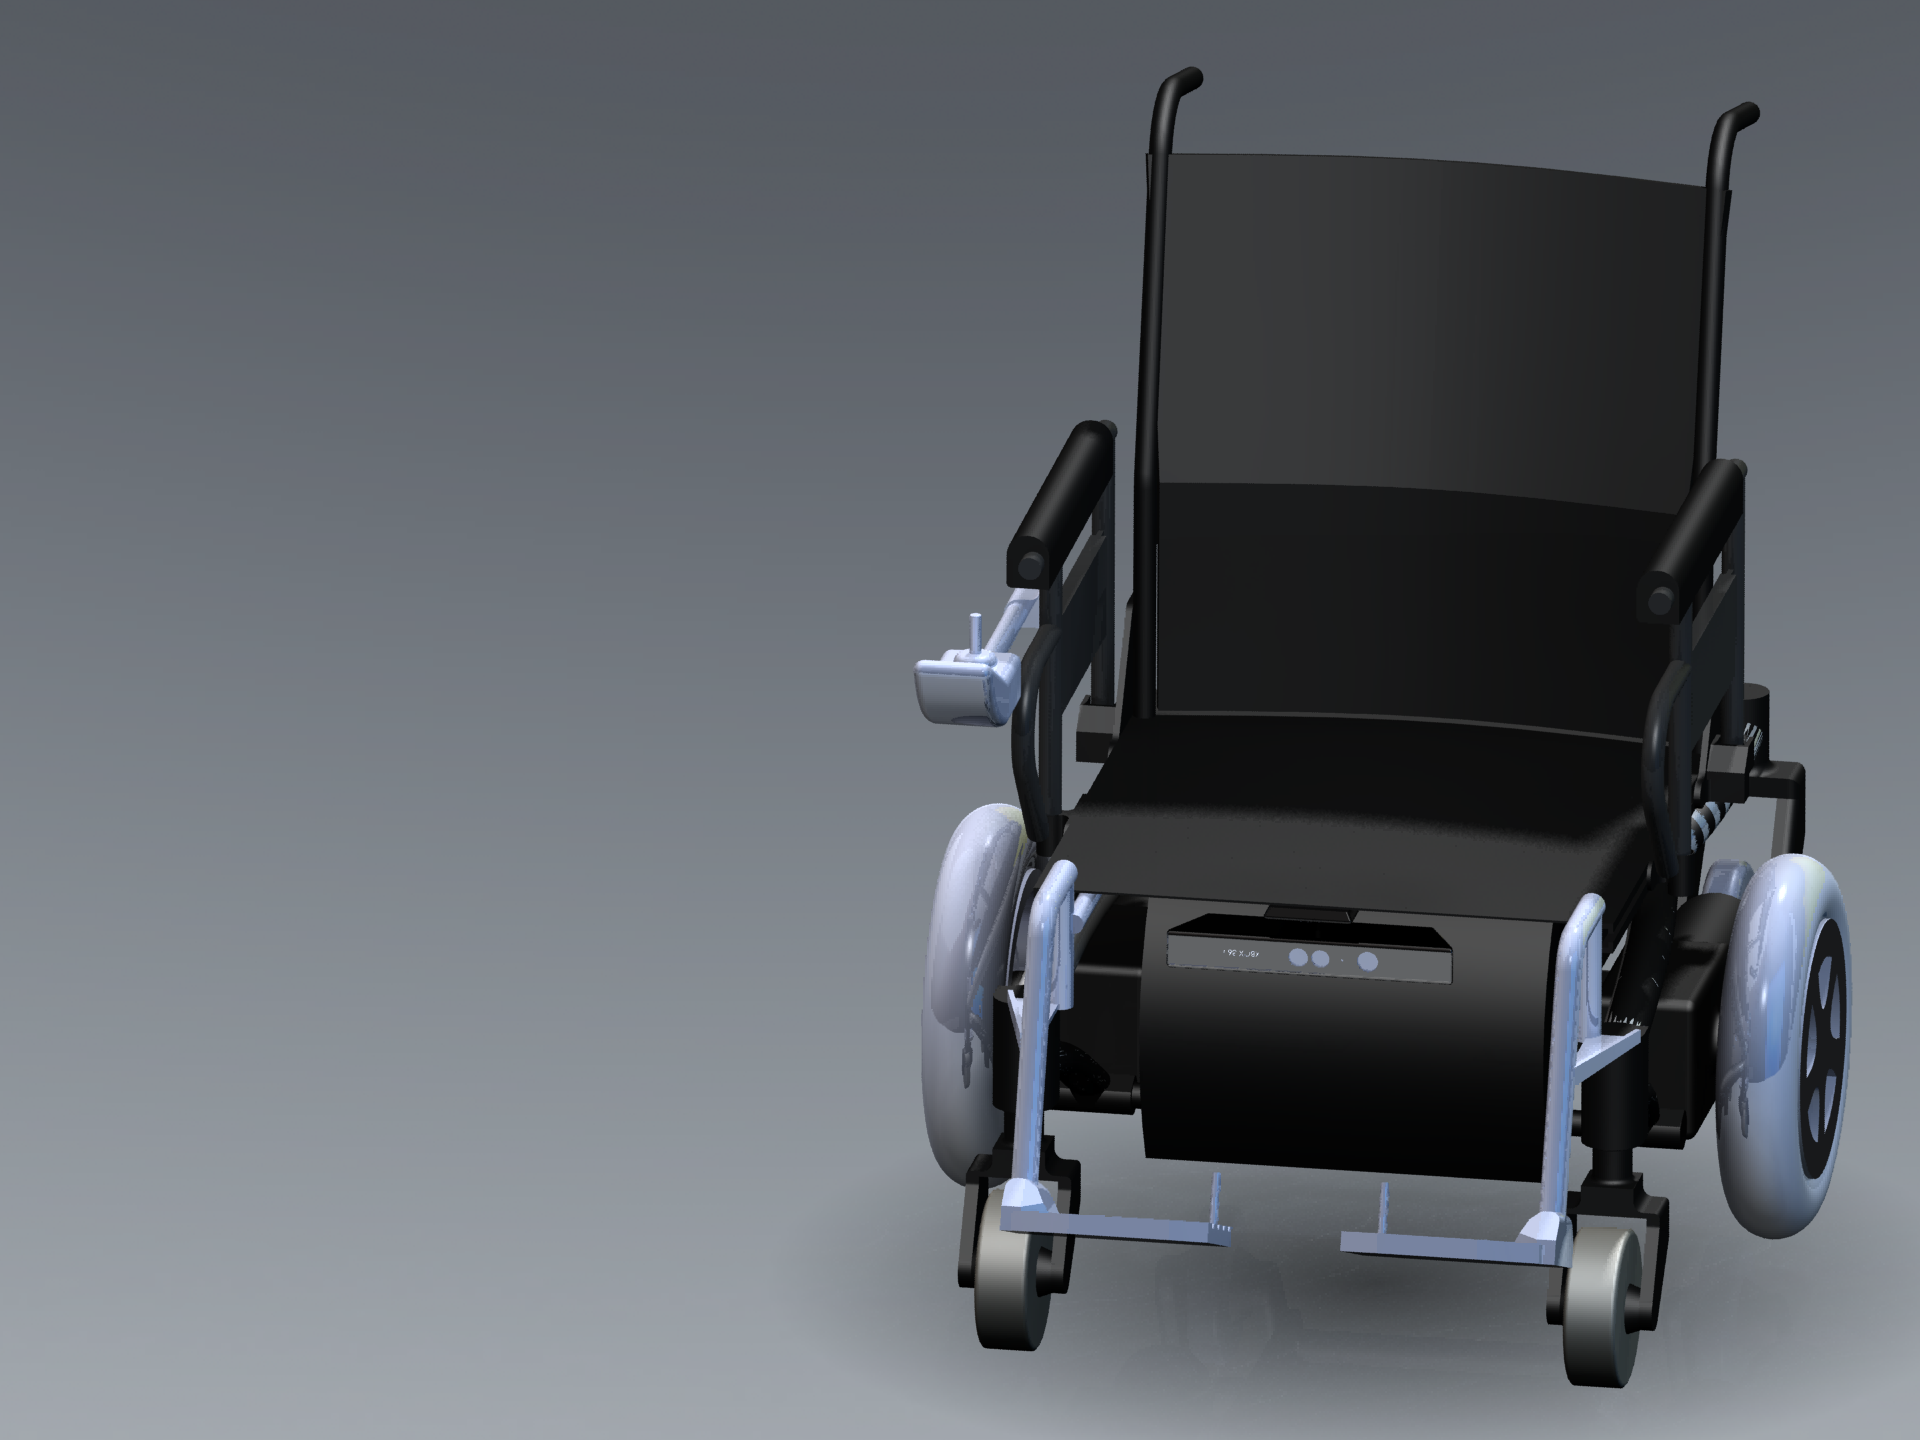
\includegraphics[scale=0.15]{WheelChair_1}
 \caption{Wheelchair Design \#1}
\end{figure}

One option was to mount the Kinect up above the user so that the user could sit in the chair with no impedances. The sensor would then have a forward looking vision viewing overtop of the user sitting in the seat. This design had the advantages of being easy to implement and much similar to the approach taken with manpowered wheel chairs with a second person pushing the chair in the appropriate direction. In addition to this the design has no inconveniences for the user since everything is mounted outside of a region where they mount or dismount. In addition to that it maintains the ability for the arms to be pushed backwards so that the user can exit via the side of the wheel chair for movements like switching from a wheel chair on to a bed or toilet.

The main disadvantage of this mounting form is that the Kinect needs to be mounted about 1m above the seat in order to meet the 95th percentile marker for males. This means that the data taken from the Kinect will need to have a transform applied to it in order to be useful to the users. Another added disadvantage is that with the Kinect mounted 1m up we add 1 m to the distance the Kinect sees all obstacles at. This is a significant reduction of the Kinects range and with it there is a reduction in the Kinects precision. One final thing is that parts of the image need to be ignored in this configuration since the Kinect cant be allowed to interpret the user as an obstacle. The 95th percentile length for the legs is that they will stick out 55 cm from the buttocks \cite{NASA}. This means that there will be a fair bit of lost data and very close proximity obstacles will be invisible to the sensor.

\subsection{Design \#2}
\begin{figure}[hbt]
 \centering
 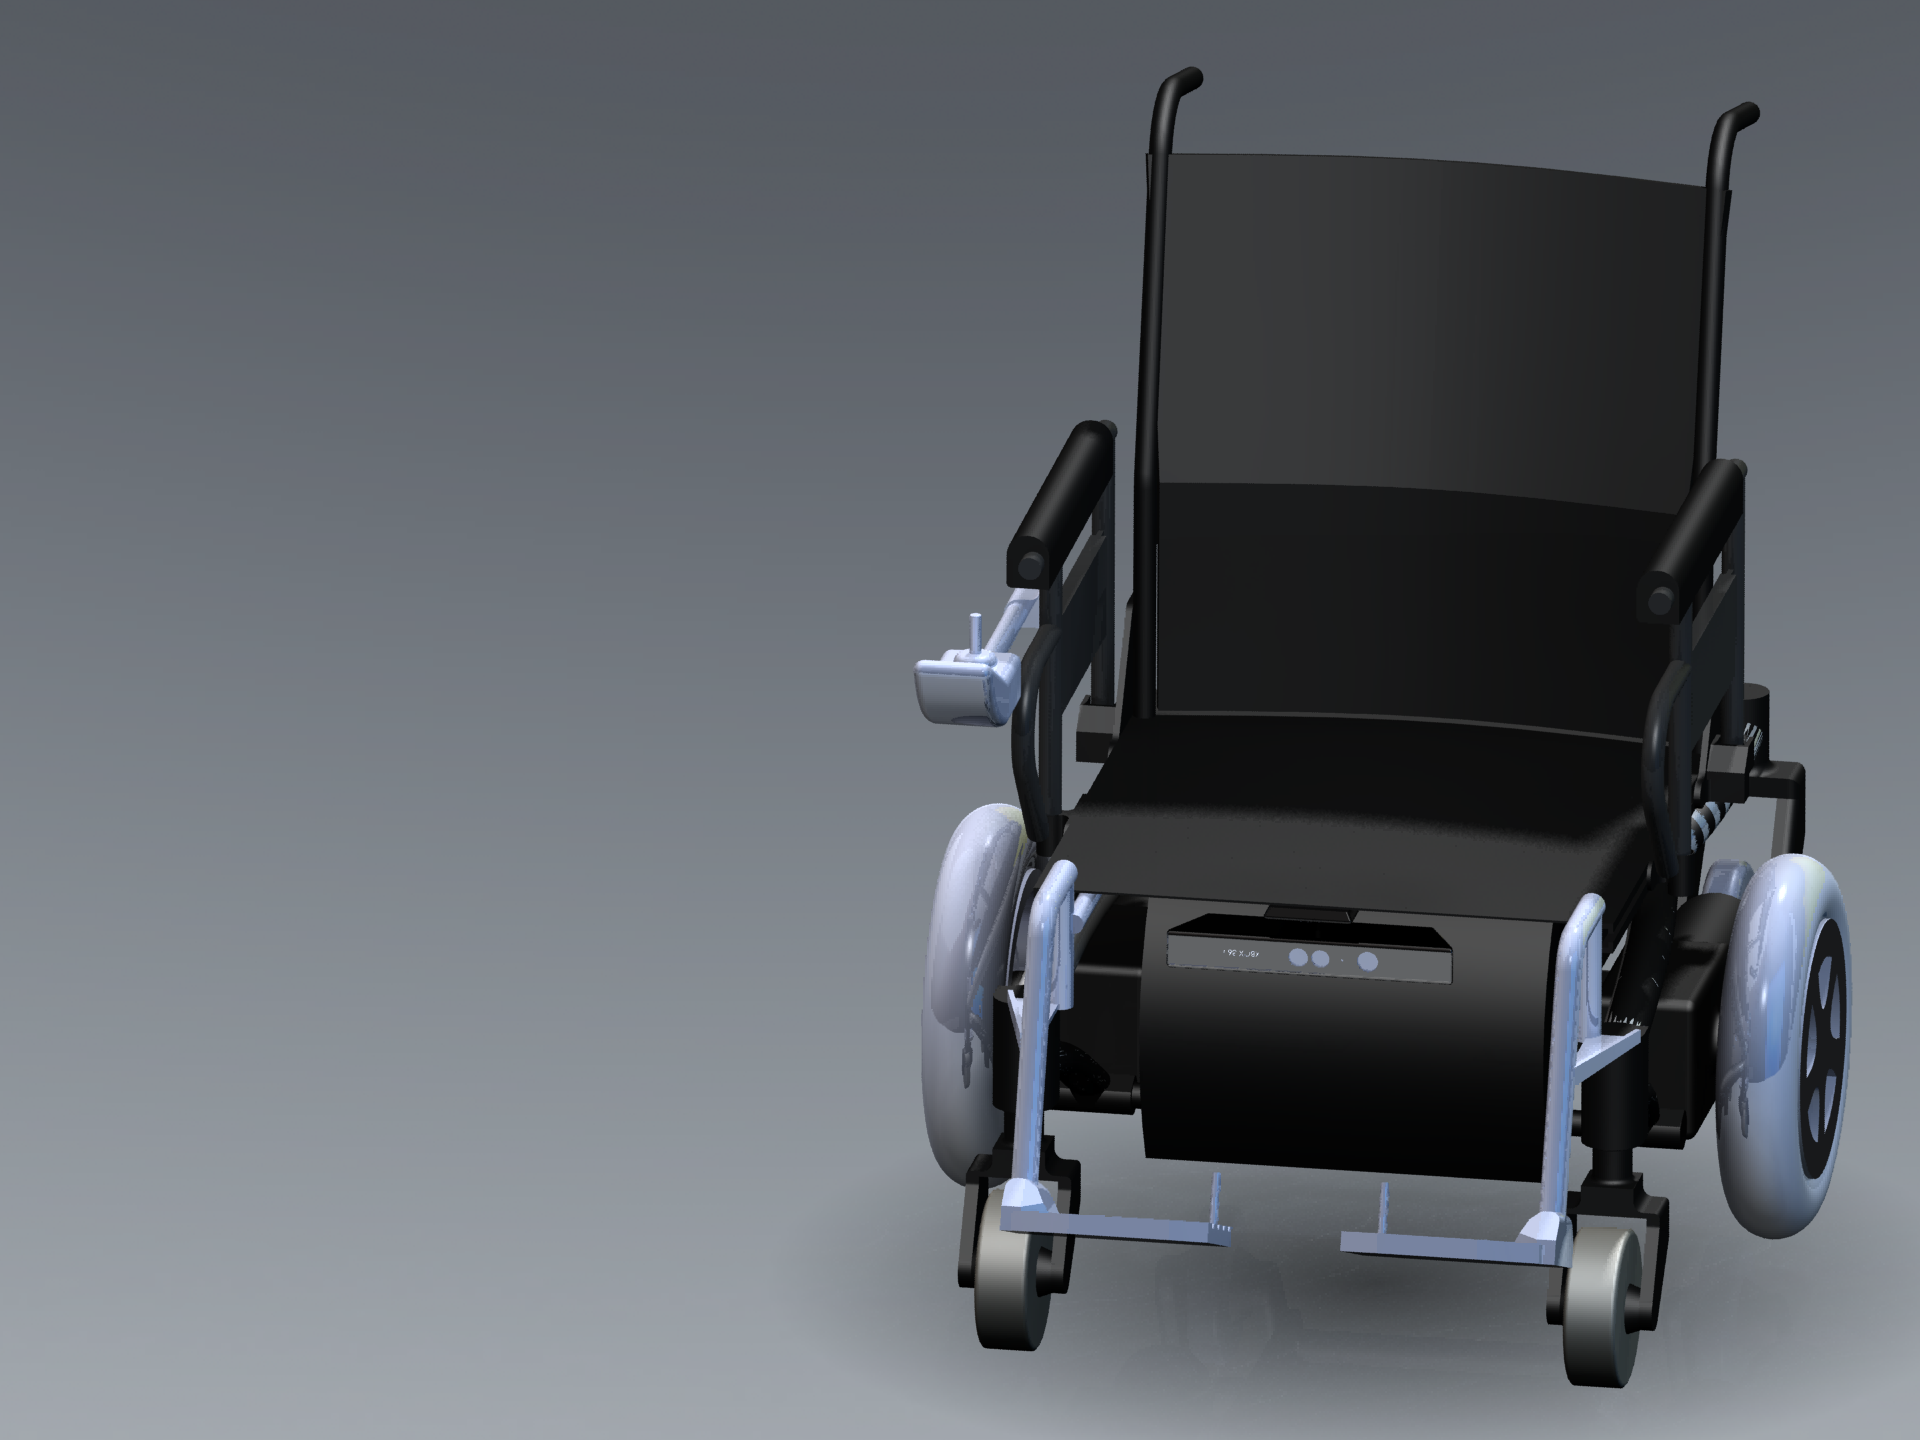
\includegraphics[scale=0.15]{WheelChair_2}
 \caption{Wheelchair Design \#2}
\end{figure}

The second design idea was to place the Kinect sensor on the bottom of the chair.  This had the advantages of being placed out of the way so the Kinect was still not in the way of the user however it places the Kinect at the same level as we would like it for sensing obstacles.It also has the advantage of being very close to the front of the chair providing the best range and precision. Lastly it also maintains the freedom of mobility that the user has with respect to pulling up the arms and exiting to a side.

The disadvantage to this is that when a user sits in the chair they often place their legs in such a way that they block the vision of the Kinect. This would effectively make all the sensors blind when the user sits in a specific orientation. Since we can’t allow this, the design was ruled out as a possible solution for where to place the Kinect sensor.

\subsection{Design \#3}
\begin{figure}[hbt]
 \centering
 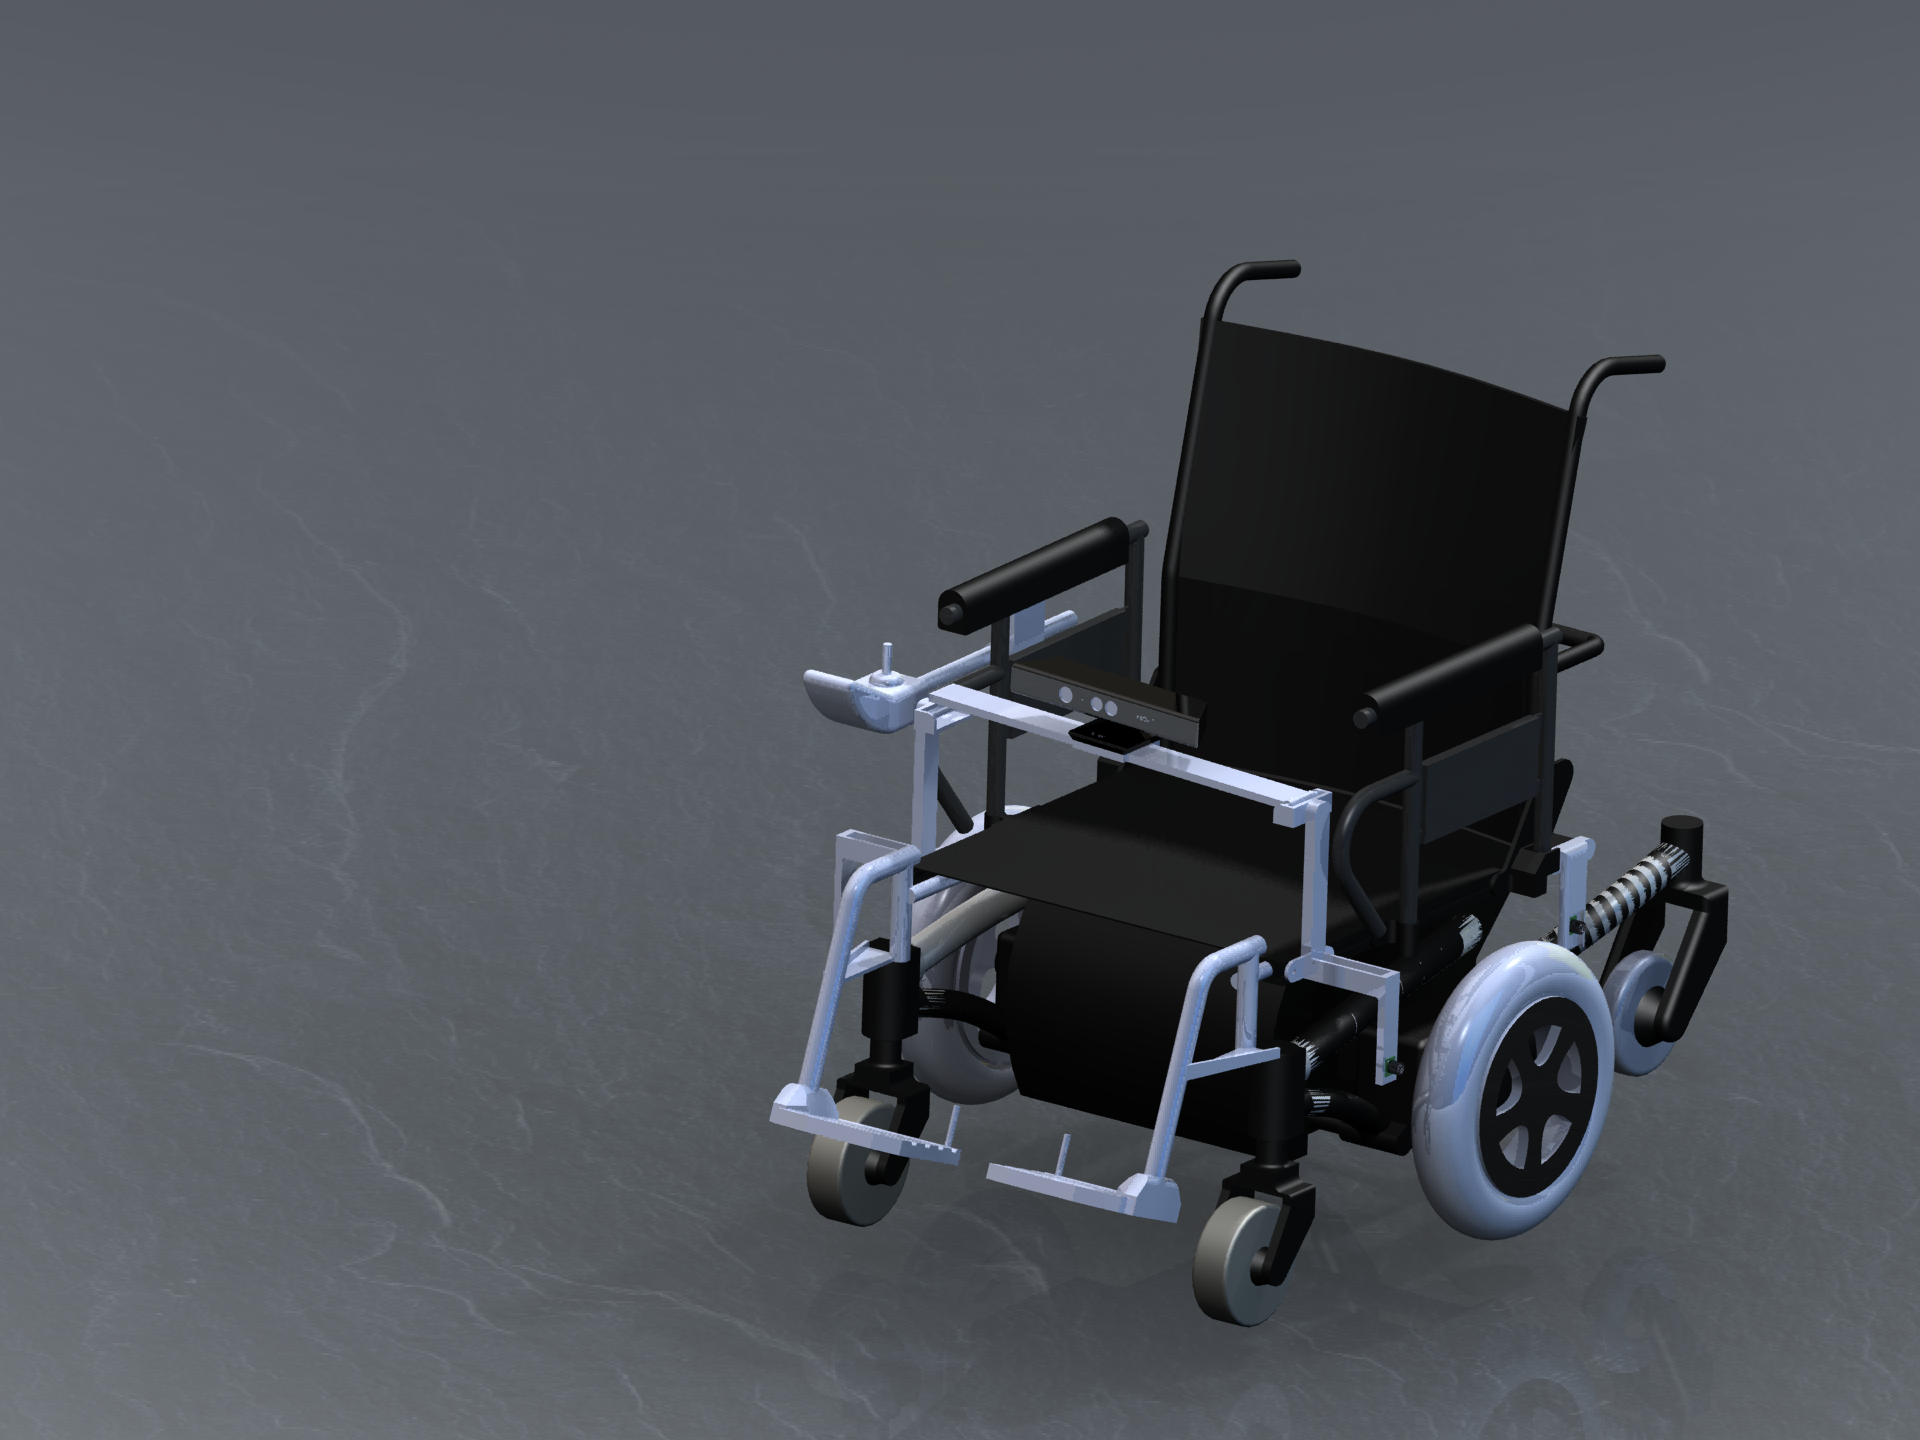
\includegraphics[scale=0.15]{WheelChair_Final}
 \caption{Wheelchair Design \#3}\label{fig:WheelChair_Final}
\end{figure}

Our third design (eventually selected as the final design, see Section \ref{MechDesSel}) made use of a concept similar to the trays found on airplanes or trains. The folding table can be lowered into position with the mounted Kinect on top of it. This has the advantage of no interference with the sensor, with it mounted at the front of the chair it makes optimal use of range and precision of the Kinect. With the sensor roughly on level with what we need it is possible to consider the occupancy map generated by the Kinect without needing to perform any transforms to get the correct orientation.

The disadvantages to this are that it is moderately more complicated mechanically since the Kinect mounting needs to be designed and made separately. There are also minor inconveniences to the user when they are attempting to get into or out of the wheel chair. It does not allow the user to move out of the chair via one of the other two sides to the chair the way the other designs do. However, the Kinect sensor has an excellent view of the floor and will be able to easily detect obstacles. Since the precision of the Kinect sensor data decreases with the square of the distance it is important to give it the best view of the environment, and since sensing quality is rated higher as a criterion than mechanical complexity this design is selected as the final design.


\section{Mechanical Design Selection} \label{MechDesSel}
Referring to the three designs mentioned above, a list of benefits and disadvantages was compilied for each design as shown in Table \ref{tab:MechDesSel}.

\begin{figure}[ht]
\centering
\begin{tabular}{|l|p{5cm}|p{5cm}|c|}
\hline
Design \# & Benefits & Disadvantages & Rating\\
\hline \hline
Design 1 &Sensor range optimal. Sensor positioning optimal. User interference minimized & User interferes with sensor readings& Unacceptable\\
\hline
Design 2 & Simplistic design. Sensor interference minimized. User interference minimized. & Sensor has shorter range. Sensor has less precision. & Acceptable\\
\hline
Design 3 & Sensor range maximized. Sensor position optimal.&Small amount of extra mechanical work. Small inconveniences to user in set up. & Acceptable (best)\\
\hline
\end{tabular}
\caption{Mechanical Design Selection}
\label{tab:MechDesSel}
\end{figure}

Based on the list of benefits and disadvantes, and the weightings of the criteria as shown in Figure \ref{fig:criteria_weighting}, the third design is selected as the final mechanical design.

\chapter{Detailed Design}

\section{System-Level Design}
\begin{figure}[hbt]
 \centering
 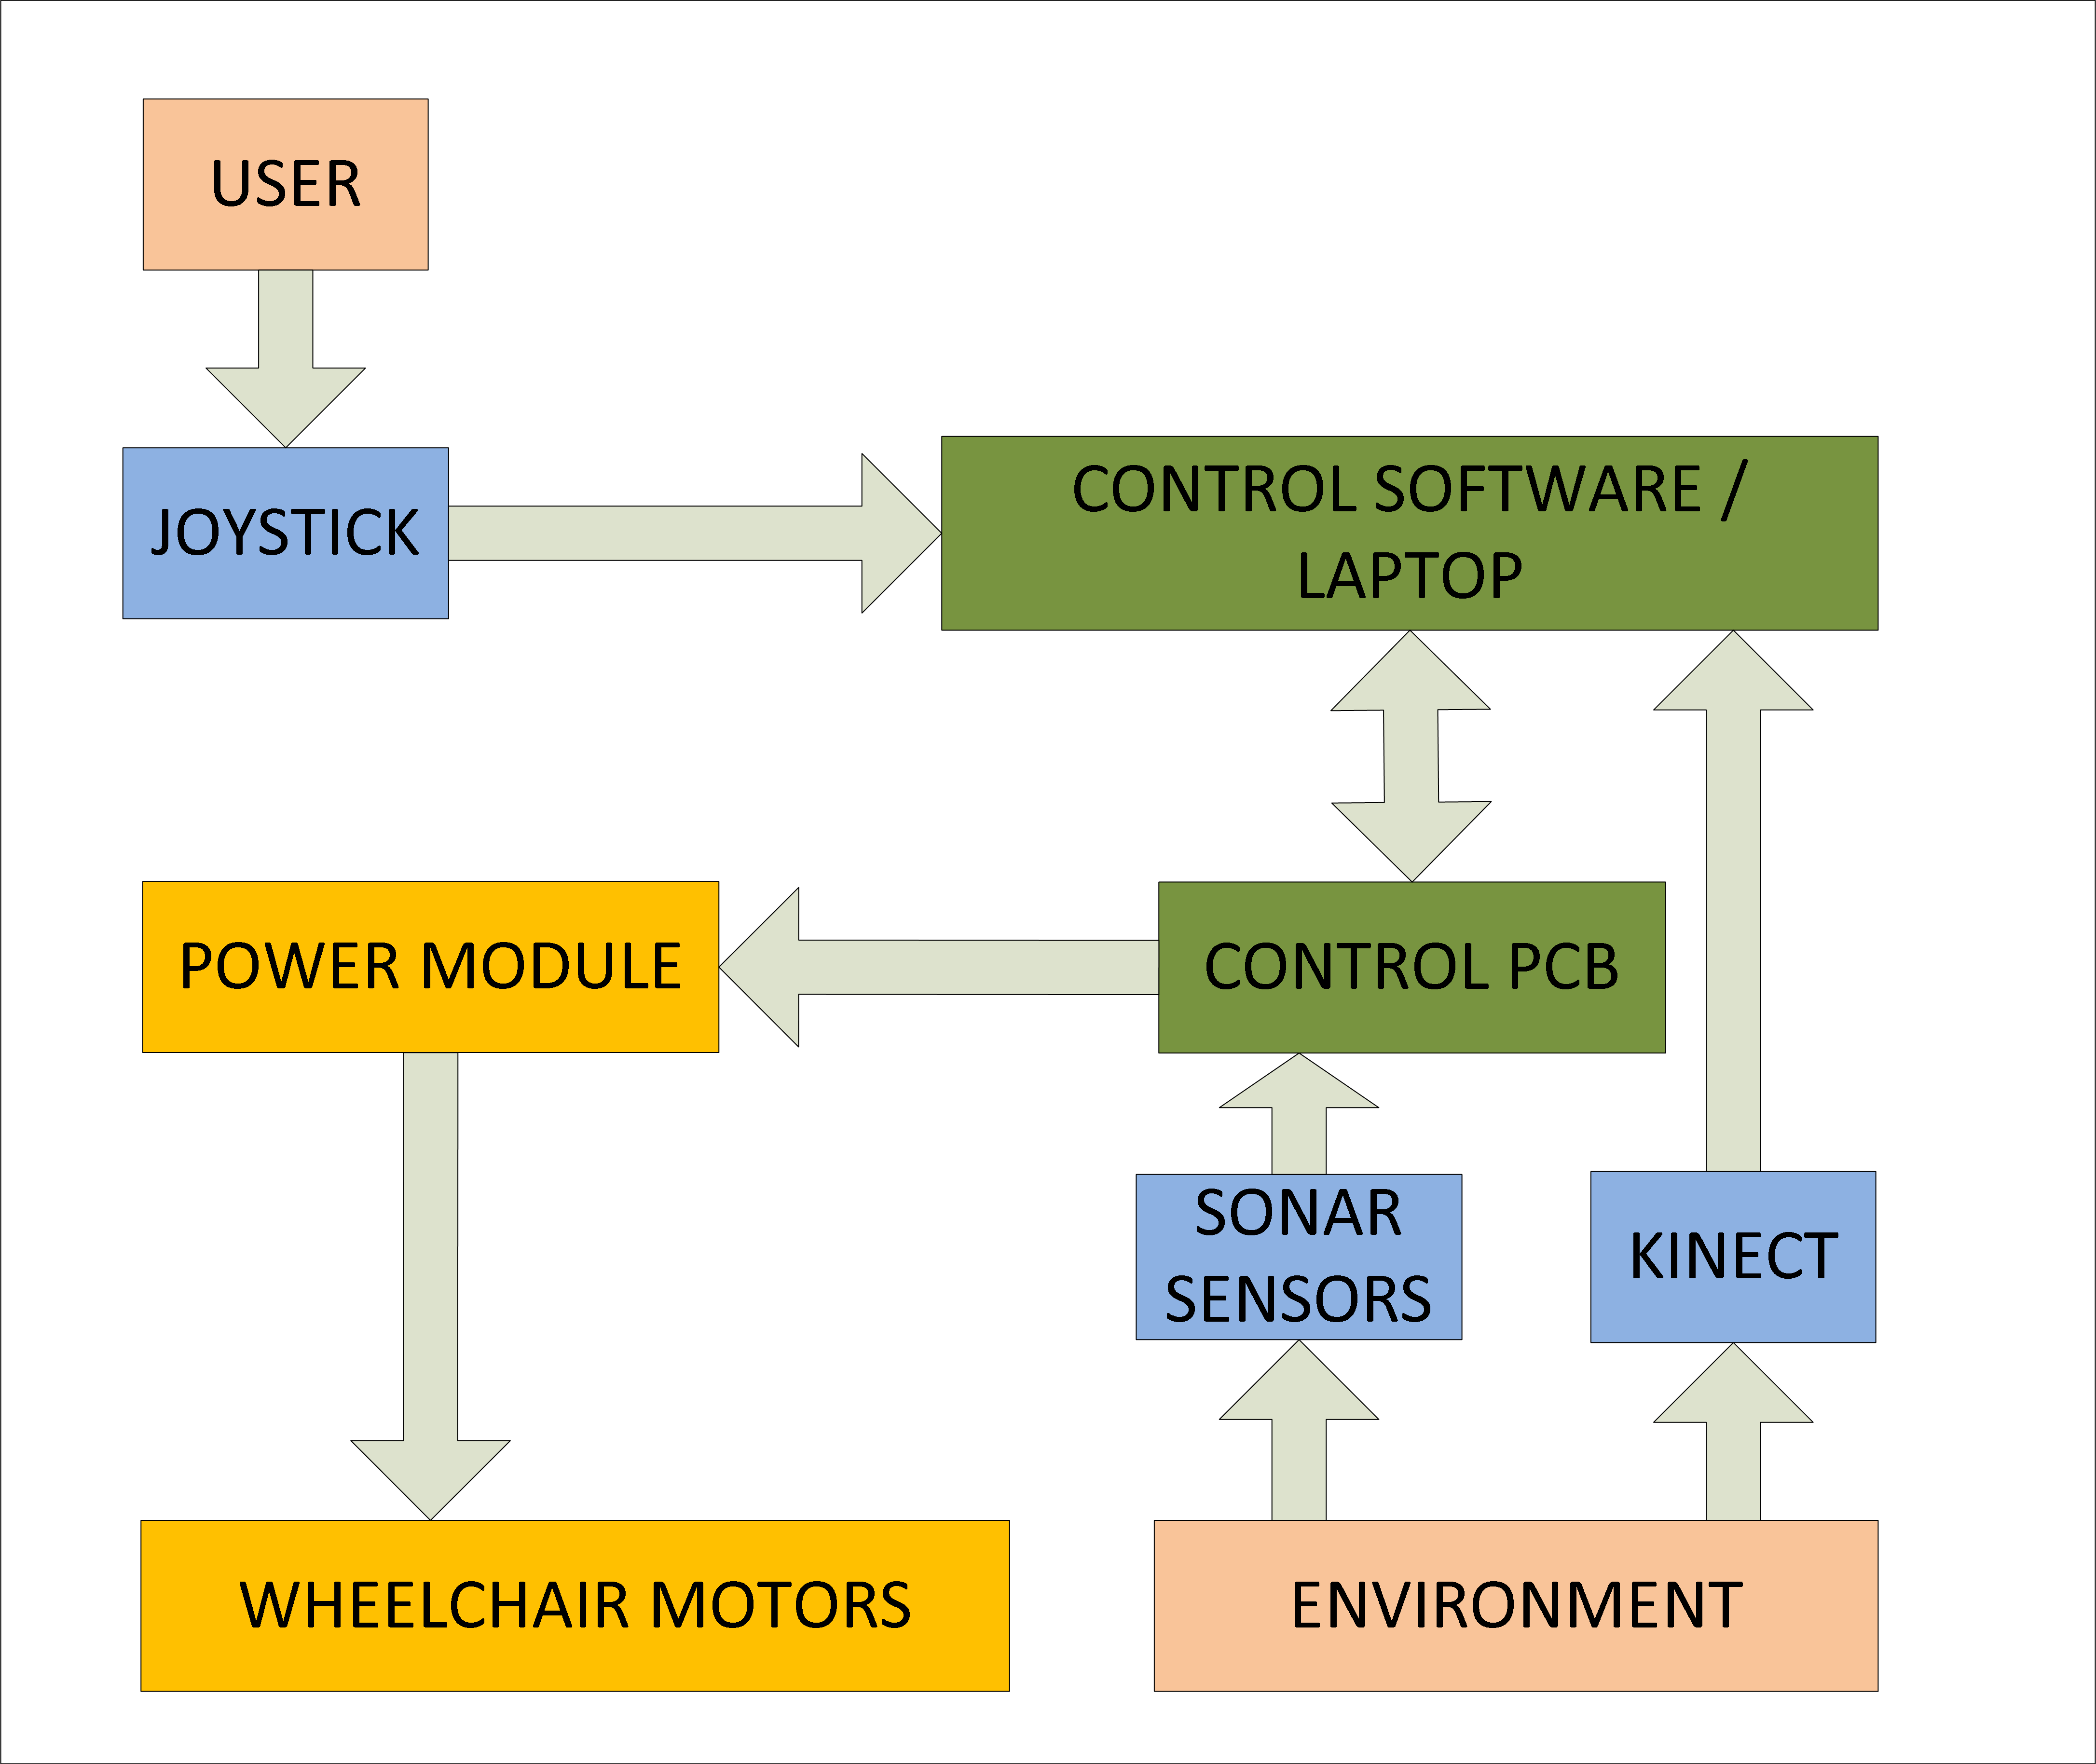
\includegraphics[scale=0.7]{System_Level}
 \caption{System Level Design}\label{fig:highlevel}
\end{figure}

Figure \ref{fig:highlevel} shows an overview of the complete system.  Pre-existing wheelchair components are highlighted in yellow, off-the-shelf components in blue, and specially designed elements in green.  The control PCB has the dual responsibility of interacting with the wheelchair motor controller and interfacing with the ultrasonic rangefinders.  The high level control software interprets sensor data, determining whether user commands are likely to result in collision, and passing velocity commands to the control PCB as appropriate.

\section{Mechanical Design}
A drawing of the final design is shown in Figure \ref{fig:WheelChair_Final}. In order to properly size the height of the tray and the sensor placements a more detailed design must be performed.

\begin{figure}[hbt]
 \centering
 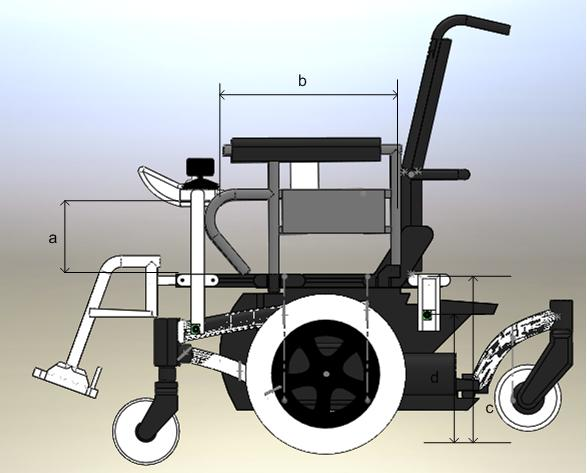
\includegraphics[scale=0.5]{WheelChair_Dimensions}
 \caption{Key Design Dimensions}\label{fig:Chair_Dims}
\end{figure}

A key set of dimensions to be considered in shown in Figure \ref{fig:Chair_Dims}. The dimensions are as follows:
\begin{enumerate}[(a)]
\item Height of the Kinect off of the surface of the chair seat
\item Distance from the back of the chair to the back of the Kinect
\item Distance from the ground to the sonar sensors mounting
\item Distance from the ground to the sonar sensor
\end{enumerate}

Based on NASA specifications for the 95th percentile male \cite{NASA} and female we can get what the dimension $a$ should be. A should be at least 12.3cm to accommodate your basic 95th percentile male. To accommodate the 5th percentile male we need 12.0cm. This means that our current design should be as shown in Appendix \ref{mech_drawings}. Since our final design model has a height of 18.42 cm there we have a safety factor of 1.49.

The distance B would be important when the Kinect interferes with the person sitting in the chair. Again relying on the information from \cite{NASA} for 95th percentile male and 5th percentile female, we can construct the data shown in Table \ref{tab:anthro_data}.

\begin{figure}[ht]
\centering
\begin{tabular}{|l|c|c|c|}
\hline
Person & Size of Stomach/Chest & Distance to Kinect & Safety Factor \\
\hline \hline
5th Percentile Male&21.8&	41.0&1.88\\
\hline
95th Percentile Male&28.2&41.0&1.45\\
\hline
5th Percentile Female&17.4&41.0&2.38\\
\hline
95th Percentile Female&23.6&41.0&1.73\\
\hline
\end{tabular}
\caption{Anthropomorphic Data}
\label{tab:anthro_data}
\end{figure}


\section{Sensor Configuration}
\begin{figure}[hbt]
 \centering
 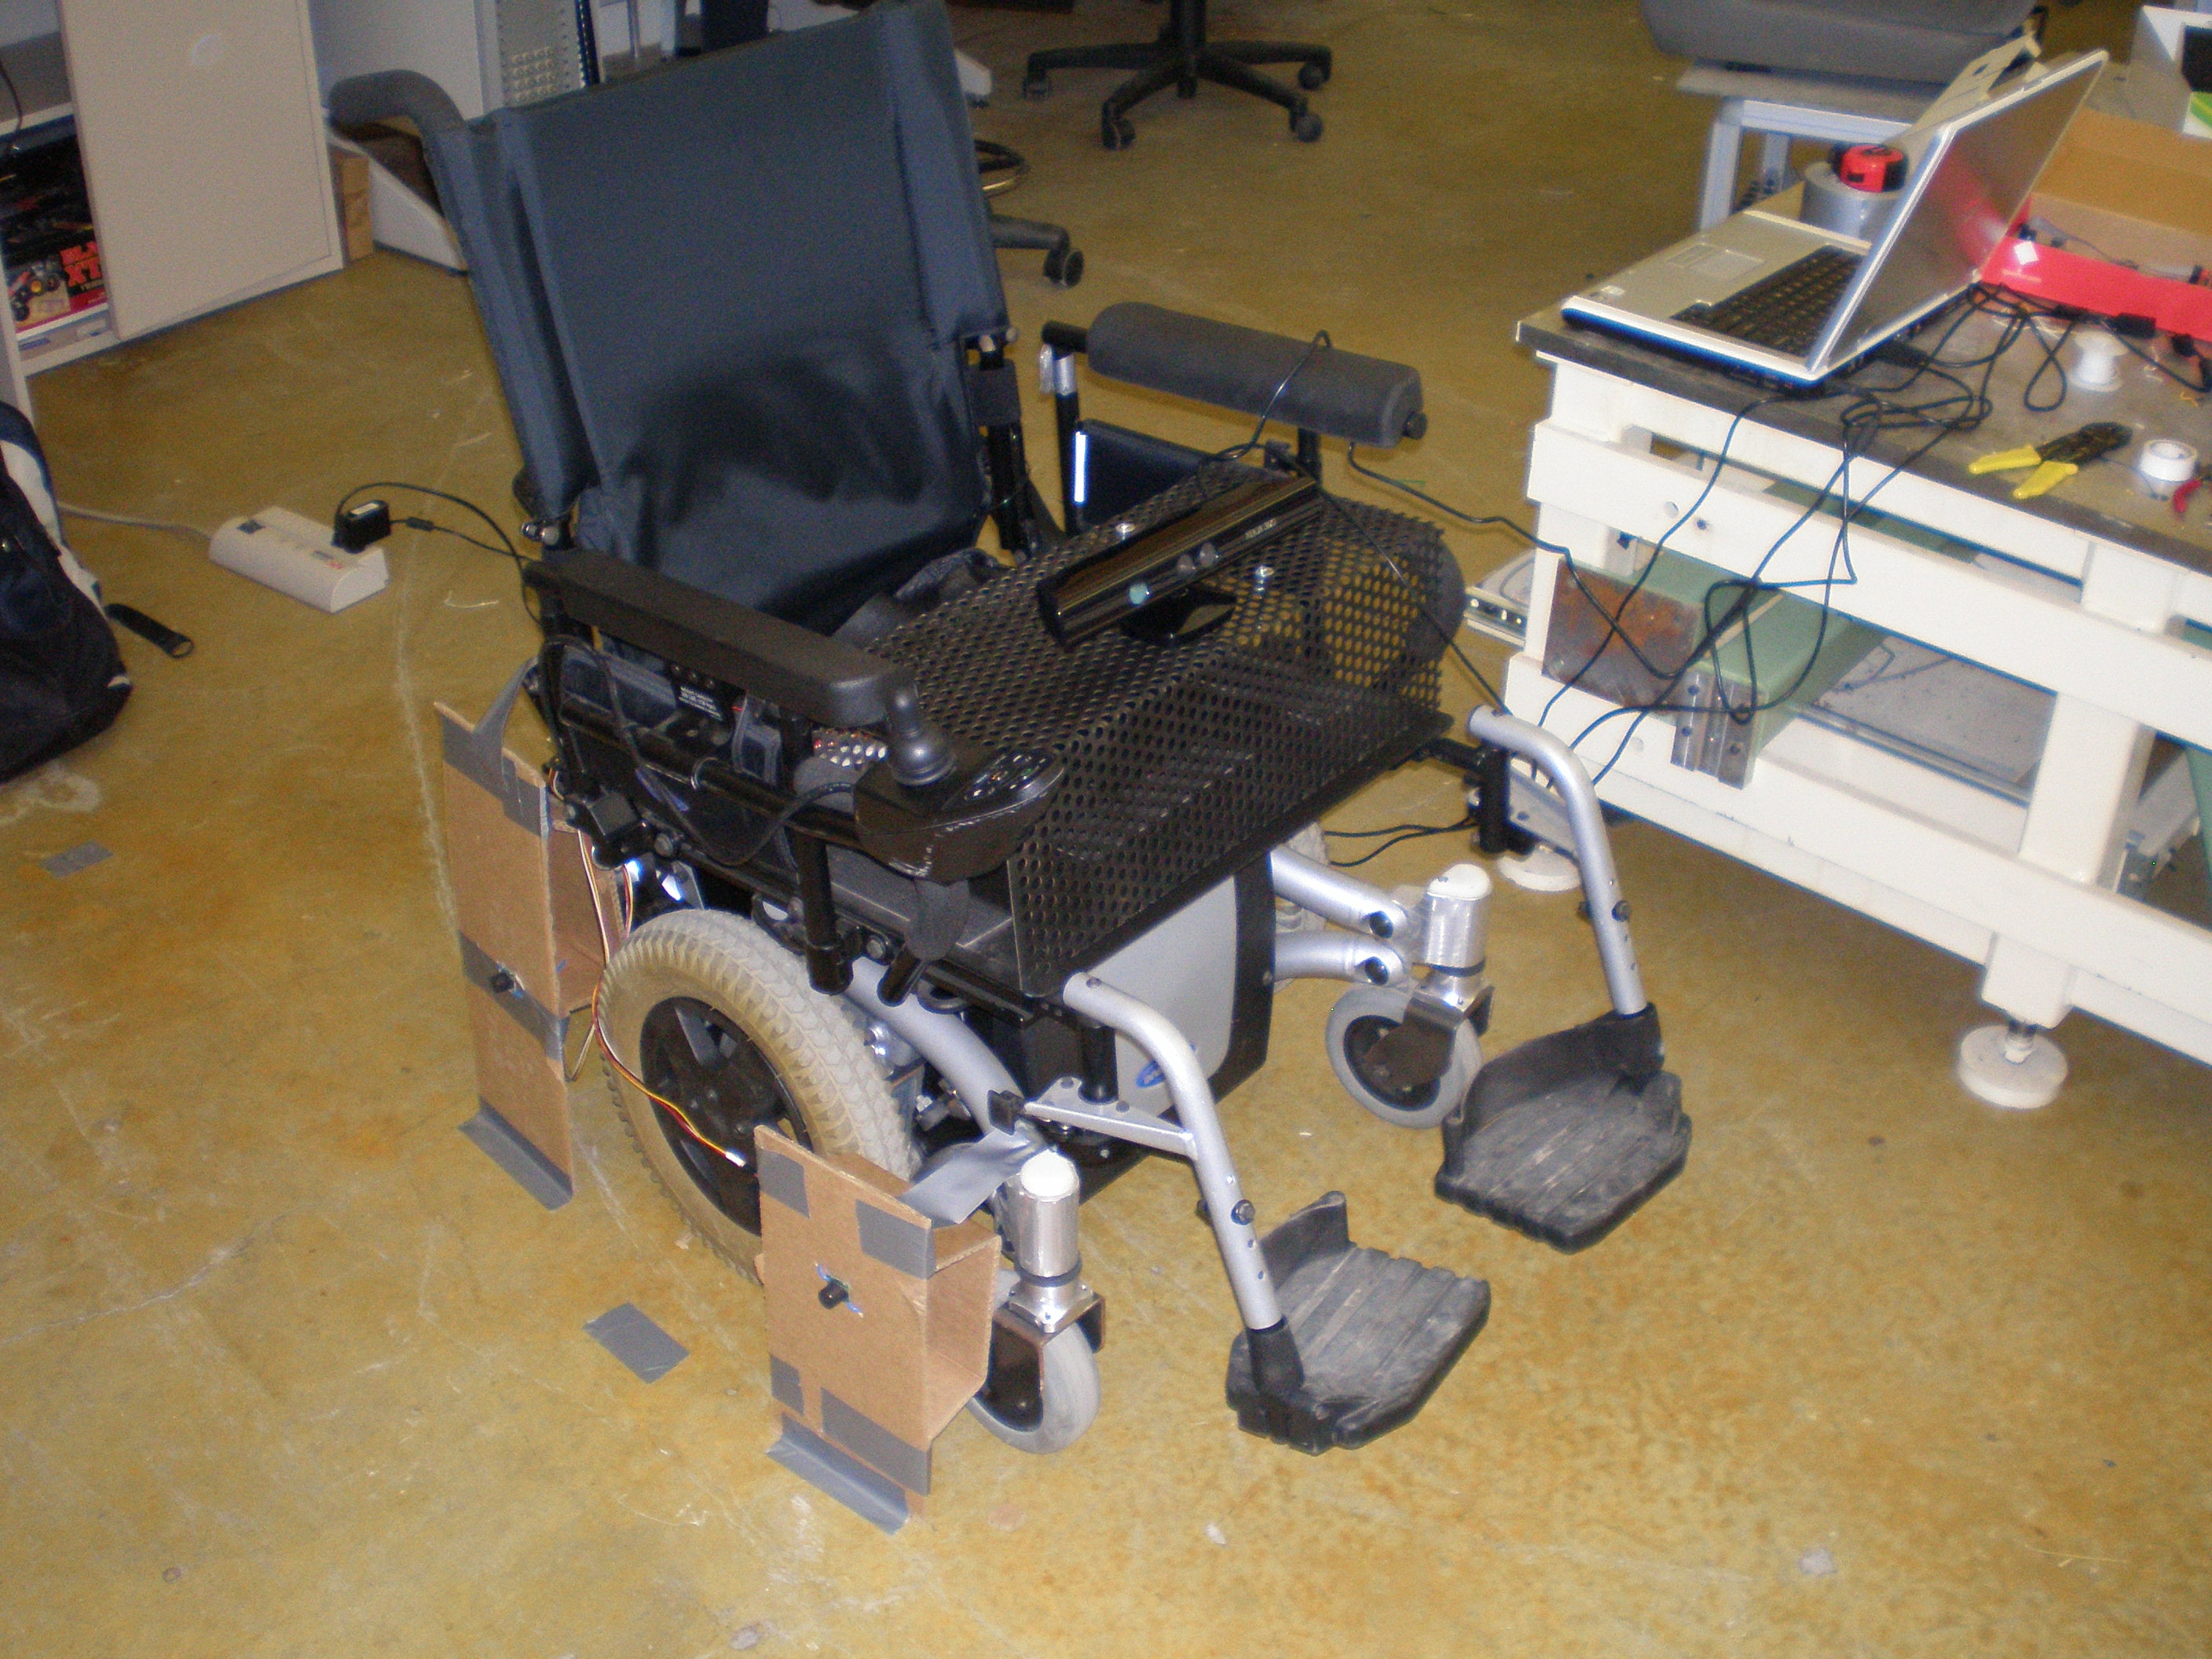
\includegraphics[scale=0.1]{testing}
 \caption{The sensor test set-up.}\label{fig:testing}
\end{figure}

\subsection{Kinect Configuration}
The Kinect sensor, based on the Primesense PS1080 System on Chip \cite{primesense}, provides a new type of depth sensing sensor. Previously projects requiring depth sensing measurements of both range and bearing (unlike ultrasonic or infrared rangers which give only range information) could use a laser rangefinder (LIDAR) or stereo-vision cameras. Laser rangefinders are both highly accurate and precise, but this comes at a very high monetary cost -- not reasonable for use in wheelchair collision avoidance technology that will be marketed to individuals and not research labs. Stereo-vision cameras require complex algorithms and lots of processing power to correspond features in images in order to identify disparities and get depth information out of this. This works out to a certain practical range -- limited by the spacing of the cameras being used and their resolution -- and is only good in areas with good lighting conditions and lots of unique features to correspond. Since the sensor is fairly new it makes sense to understand how it works, and what its accuracy and precision is, before determining the best final configuration.

The Primsense depth-sensor solution is shown in Figure \ref{fig:primesense_solution}. The Kinect presents something of a combination between the lidar and the stereo vision depth mapping techniques, sending out coded infrared light (similar to a lidar) and reading back the response on a standard CMOS image sensor (which keeps things very cheap). The solution does all its processing on board the PS1080, and sends the fully-processed depth map information back to the host. The result is reasonable accuracy and precision (for this application), and low price. Note that while the Xbox Kinect from Microsoft is being used for the prototype of this collision aviodance project, there are other manufacturers of depth sensors using the Primesense technology on the market that could eventually be used to reduce cost for production purposes.

\begin{figure}[hbt]
 \centering
 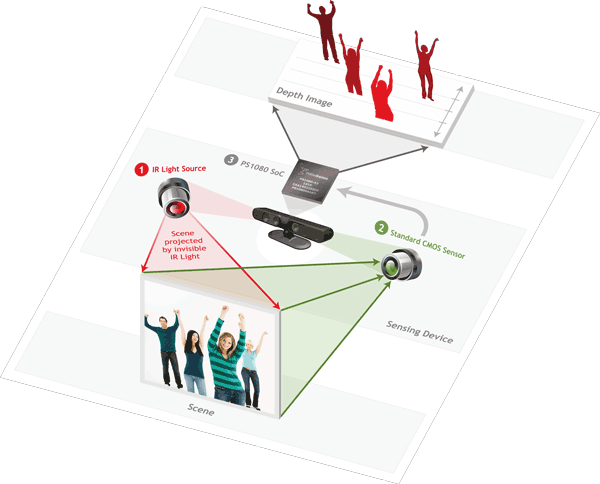
\includegraphics[scale=0.35]{PrimeSensor_Depth_Diagram}
 \caption{The Primesense system \cite{primesense}} \label{fig:primesense_solution}
\end{figure}

The Kinect comes with a set of camera calibration parameters, and the software available from OpenNI \cite{OpenNI} and the Robot Operating System (ROS) \cite{ROS} package that supports the Kinect have gone to great lengths to provide a good calibration for the depth camera. The result is that the accuracy of the sensor is within  $\pm 1$ 1 cm of the true measurement, and with custom calibration with $\pm 1$ mm over its range of operation \cite{kinect_prec}.

The precision is less good (though still not bad at all) and increases with the square of distance. This is shown in Figure \ref{fig:kinect_precision} provided by \cite{kinect_prec}. However, for the application of collision avoidance very high precision data is not required, and we can see that even out to 2 meters of range the 95th percentile of data falls with 2.5 cm of the true range. It will quickly fall off in precision with range, but the wheelchair does not need to react very quickly to data that is farther away, and in tight spots the wheelchair will be close to obstacles and hence get very precise data from sensor.

\begin{figure}[hbt]
 \centering
 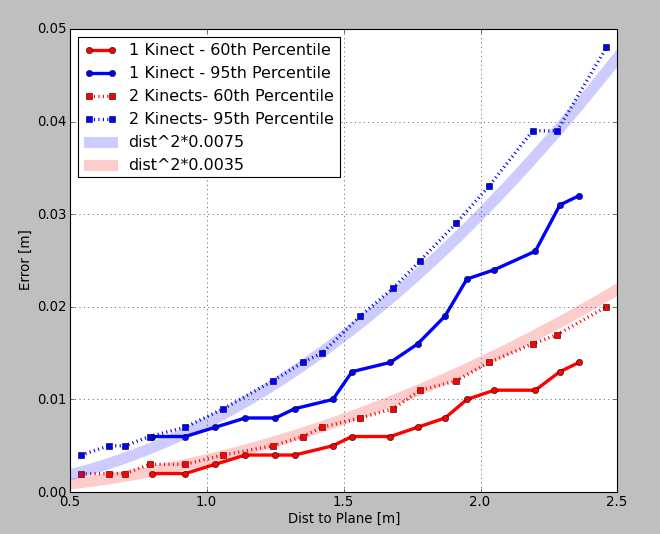
\includegraphics[scale=0.35]{kinect_precision}
 \caption{Kinect Sensor Precision \cite{kinect_prec}} \label{fig:kinect_precision}
\end{figure}

To prove out the operation of the Kinect sensor, the test setup shown in Figure \ref{fig:testing}. The authors stood in front of the camera at a few meters of range and a set of data was gathered. This data is shown in the format of a point cloud \cite{point_clouds} in Figure \ref{fig:groupPCL}. A point cloud is a set of (X,Y,Z) coordinates that represents the depth (Z) of a point at each (X,Y) coordinate on the map. This is provided to us in meters, being converted from the camera perspective to the world (X,Y,Z) frame transparently by using ROS and the OpenNI Kinect node that comes as  "node", a program that operates in the ROS environment.

\begin{figure}[hbt]
 \centering
 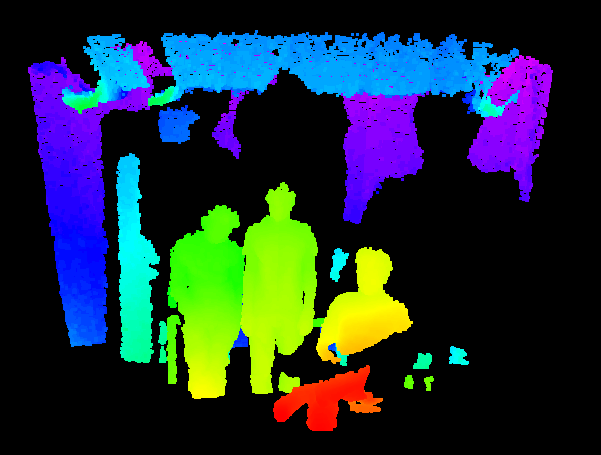
\includegraphics[scale=0.35]{group_pointcloud}
 \caption{Kinect Point Cloud Sample} \label{fig:groupPCL}
\end{figure}

The problem with this point cloud data is that it can include floor and ceiling measurements (as seen in Figure \ref{fig:groupPCL} that are clearly not obstacles. Also, if the camera is not pointing parallel to the floor the "world" coordinate frame axes used to construct the point cloud will not be lined up with ground plane (a level floor in the case of a wheelchair).

The solution is to first transform the point cloud data into the true world coodinate frame using a simple rotation matrix. The desired rotation can either be read from the accelerometer in the Kinect sensor (by measuring the gravity vector), finding a plane of best fit using an image of the floor, or just calibrating the sensor once at the time of manufacture when it is fixed to the wheelchair. Then only a slice of the point cloud is considered, the one above the floor plane but below what would be considered the top of the wheelchair. This slice is projected onto a course grid where any points within a box cause an object to be indicated, and otherwise the box is considered free space. The occupancy grid for Figure \ref{fig:groupPCL} is shown in Figure \ref{fig:groupOccupancy}.

\begin{figure}[hbt]
 \centering
 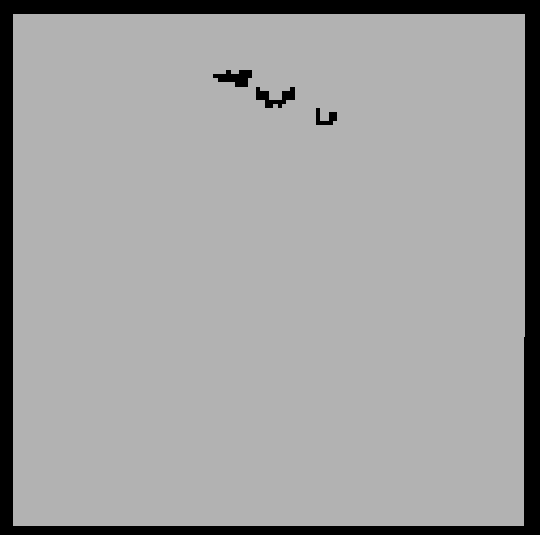
\includegraphics[scale=0.35]{group_occupancy}
 \caption{Kinect Occupancy Grid Sample} \label{fig:groupOccupancy}
\end{figure}

The occupancy grid shows free space (grey) and obstacles (black). Comparing Figure \ref{fig:groupPCL} to Figure \ref{fig:groupOccupancy} we can see the torsos of two individuals and the head of a third shown in the occupancy map. This is because the slice closen to be projected onto the grid was a 30 cm range about the center of the image, at approximately the head height of the seated individual. In practice, this range with be tuned to avoid accidental measurments from the floor and extend up to the height of the wheelchair to reject false obstacles such as the floors and ceilings.

This proves the concept works well, and only some tuning of the constants will be required to integrate the Kinect with the final prototype.

\section{Rangefinder Configuration}
SONAR sensors which were available on-hand were used to test a number of configurations.  The sensors used were the MaxBotix LV-EZ4.  These sensors are designed to be sensitive to object only within a cylindrical region of about 60 cm diameter \cite{lv-ez4}.  

Figures \ref{sonar_1} - \ref{sonar_3} show the results of testing with the LV-EZ4.  Unsurprisingly, area coverage is poor with the narrow-beam sensor.  The best results are observed in figure \ref{sonar_2}, where the forward field is fully covered.

\begin{figure}[hbt]
 \centering
 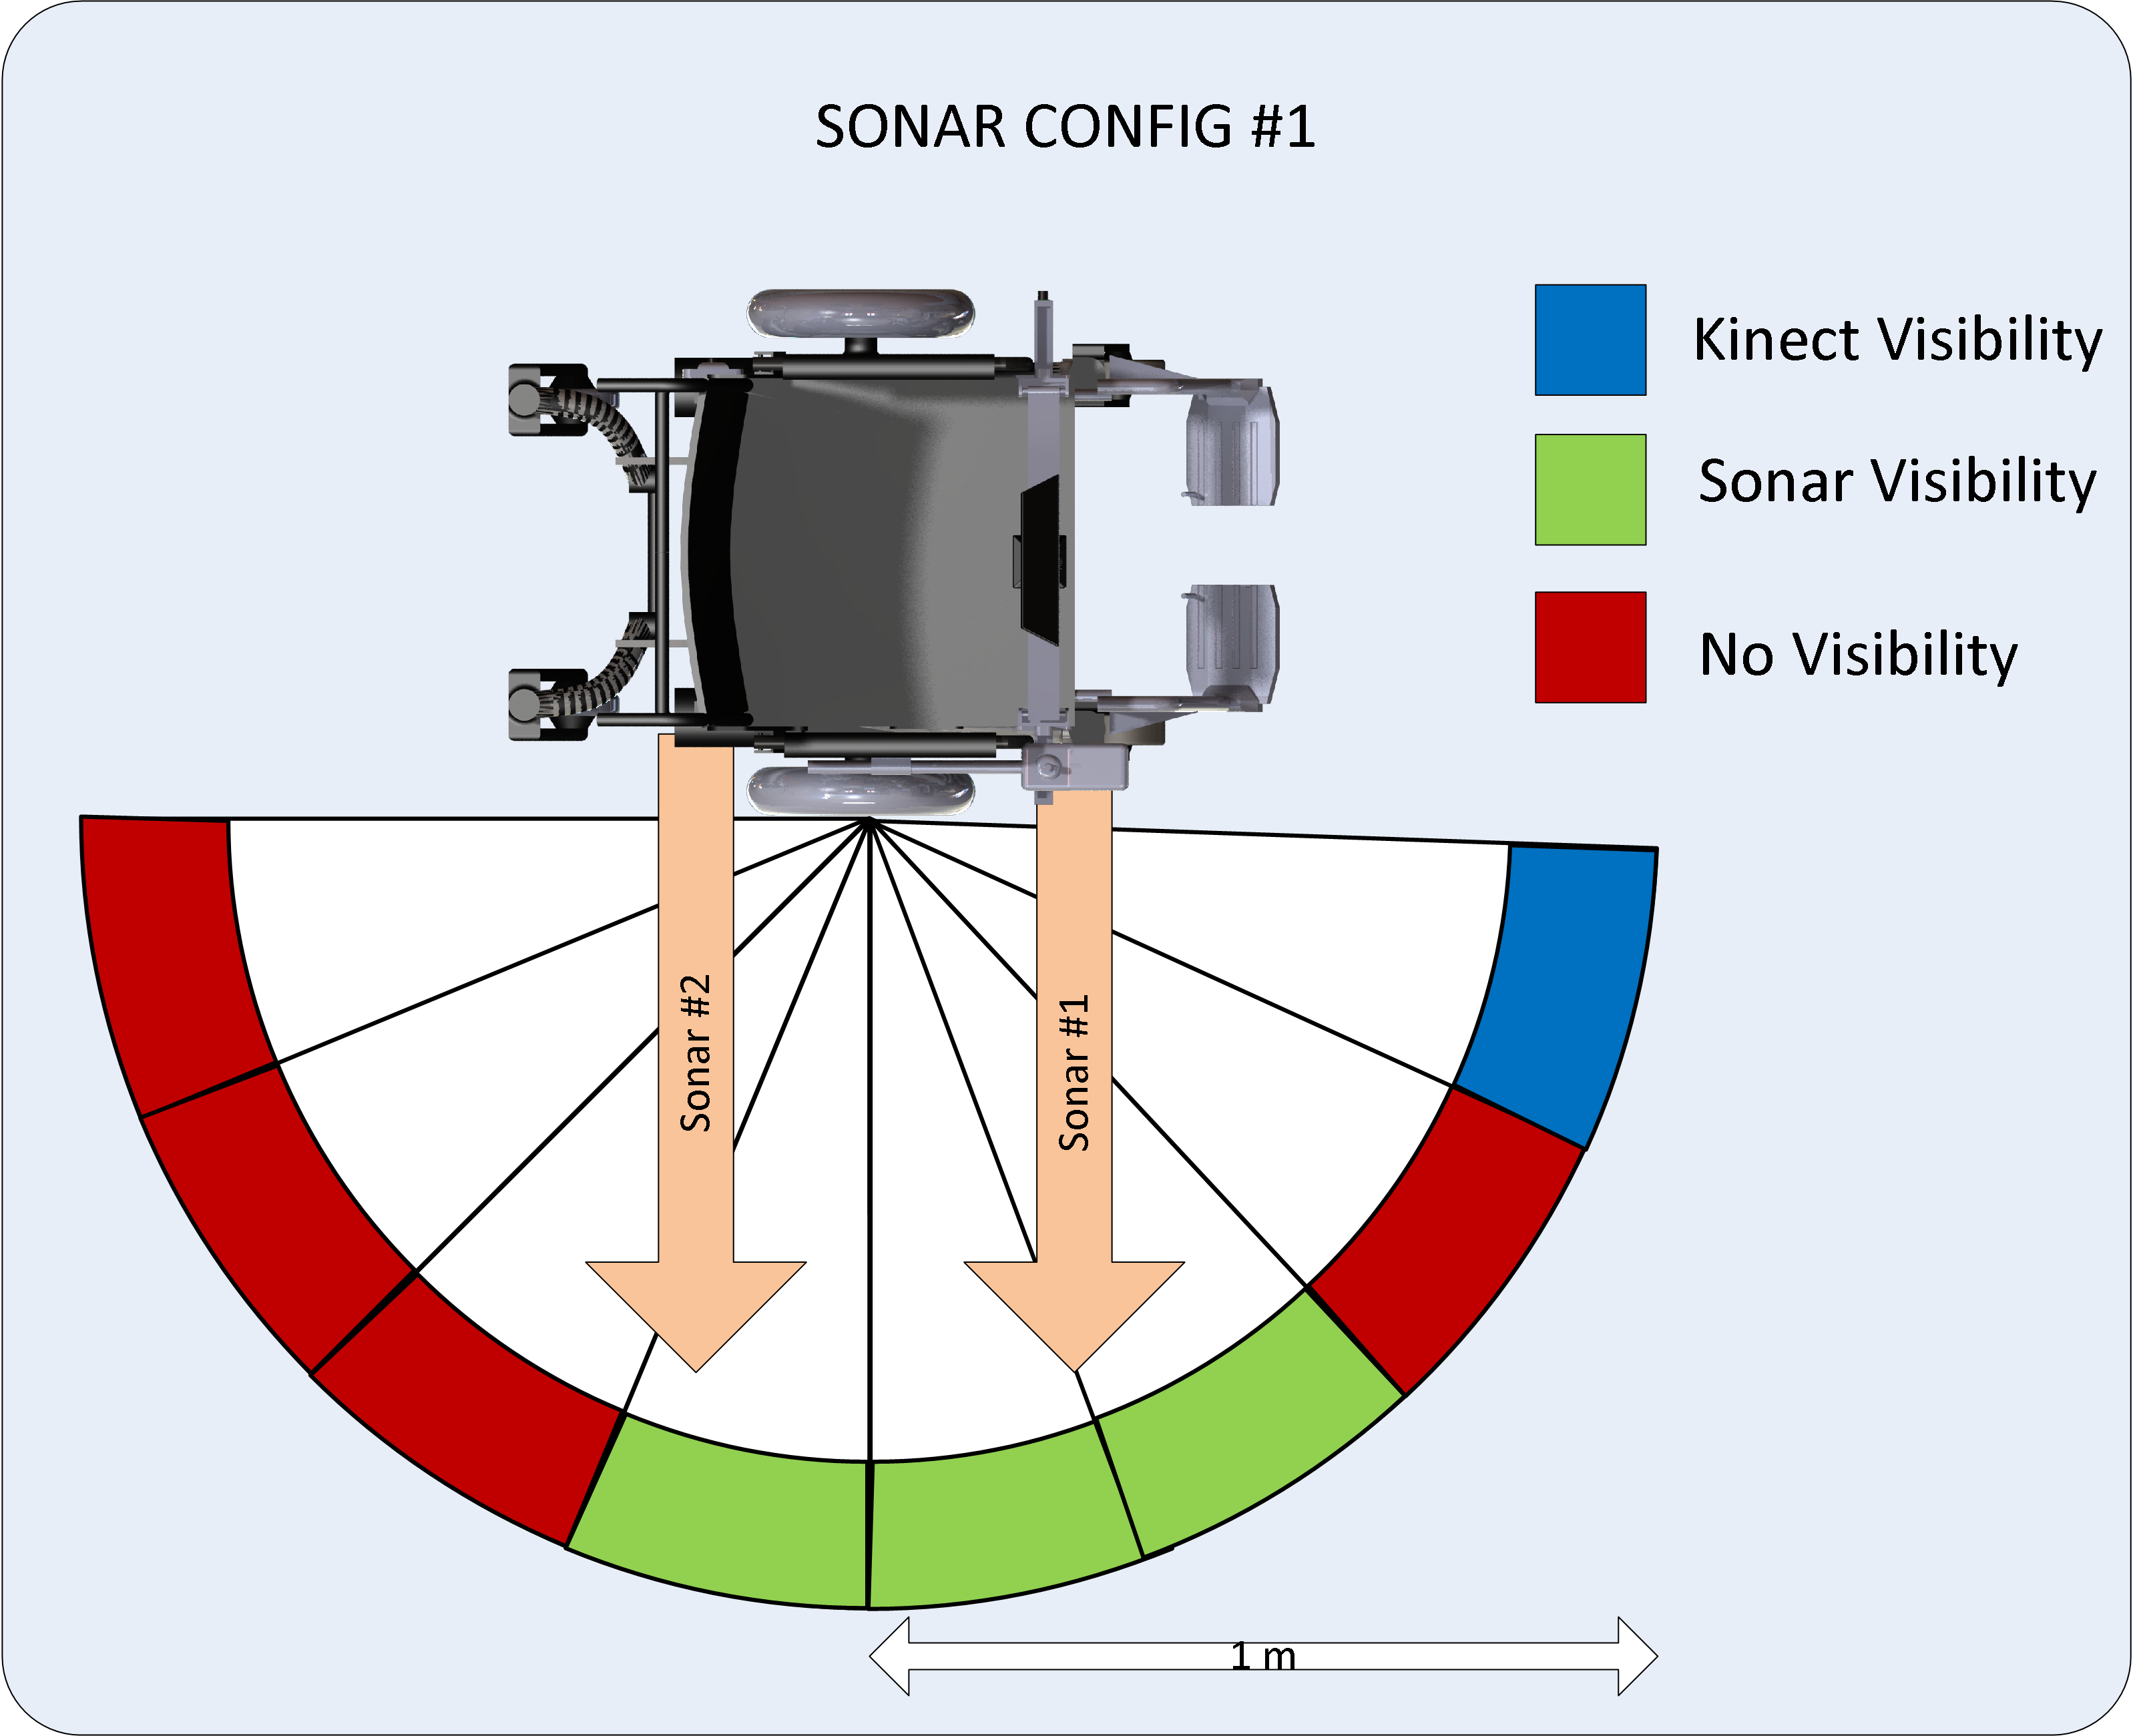
\includegraphics[scale=0.6]{SONAR_Config1.png}
 \caption{SONAR test configuration 1.}
 \label{sonar_1}
\end{figure}

\begin{figure}[hbt]
 \centering
 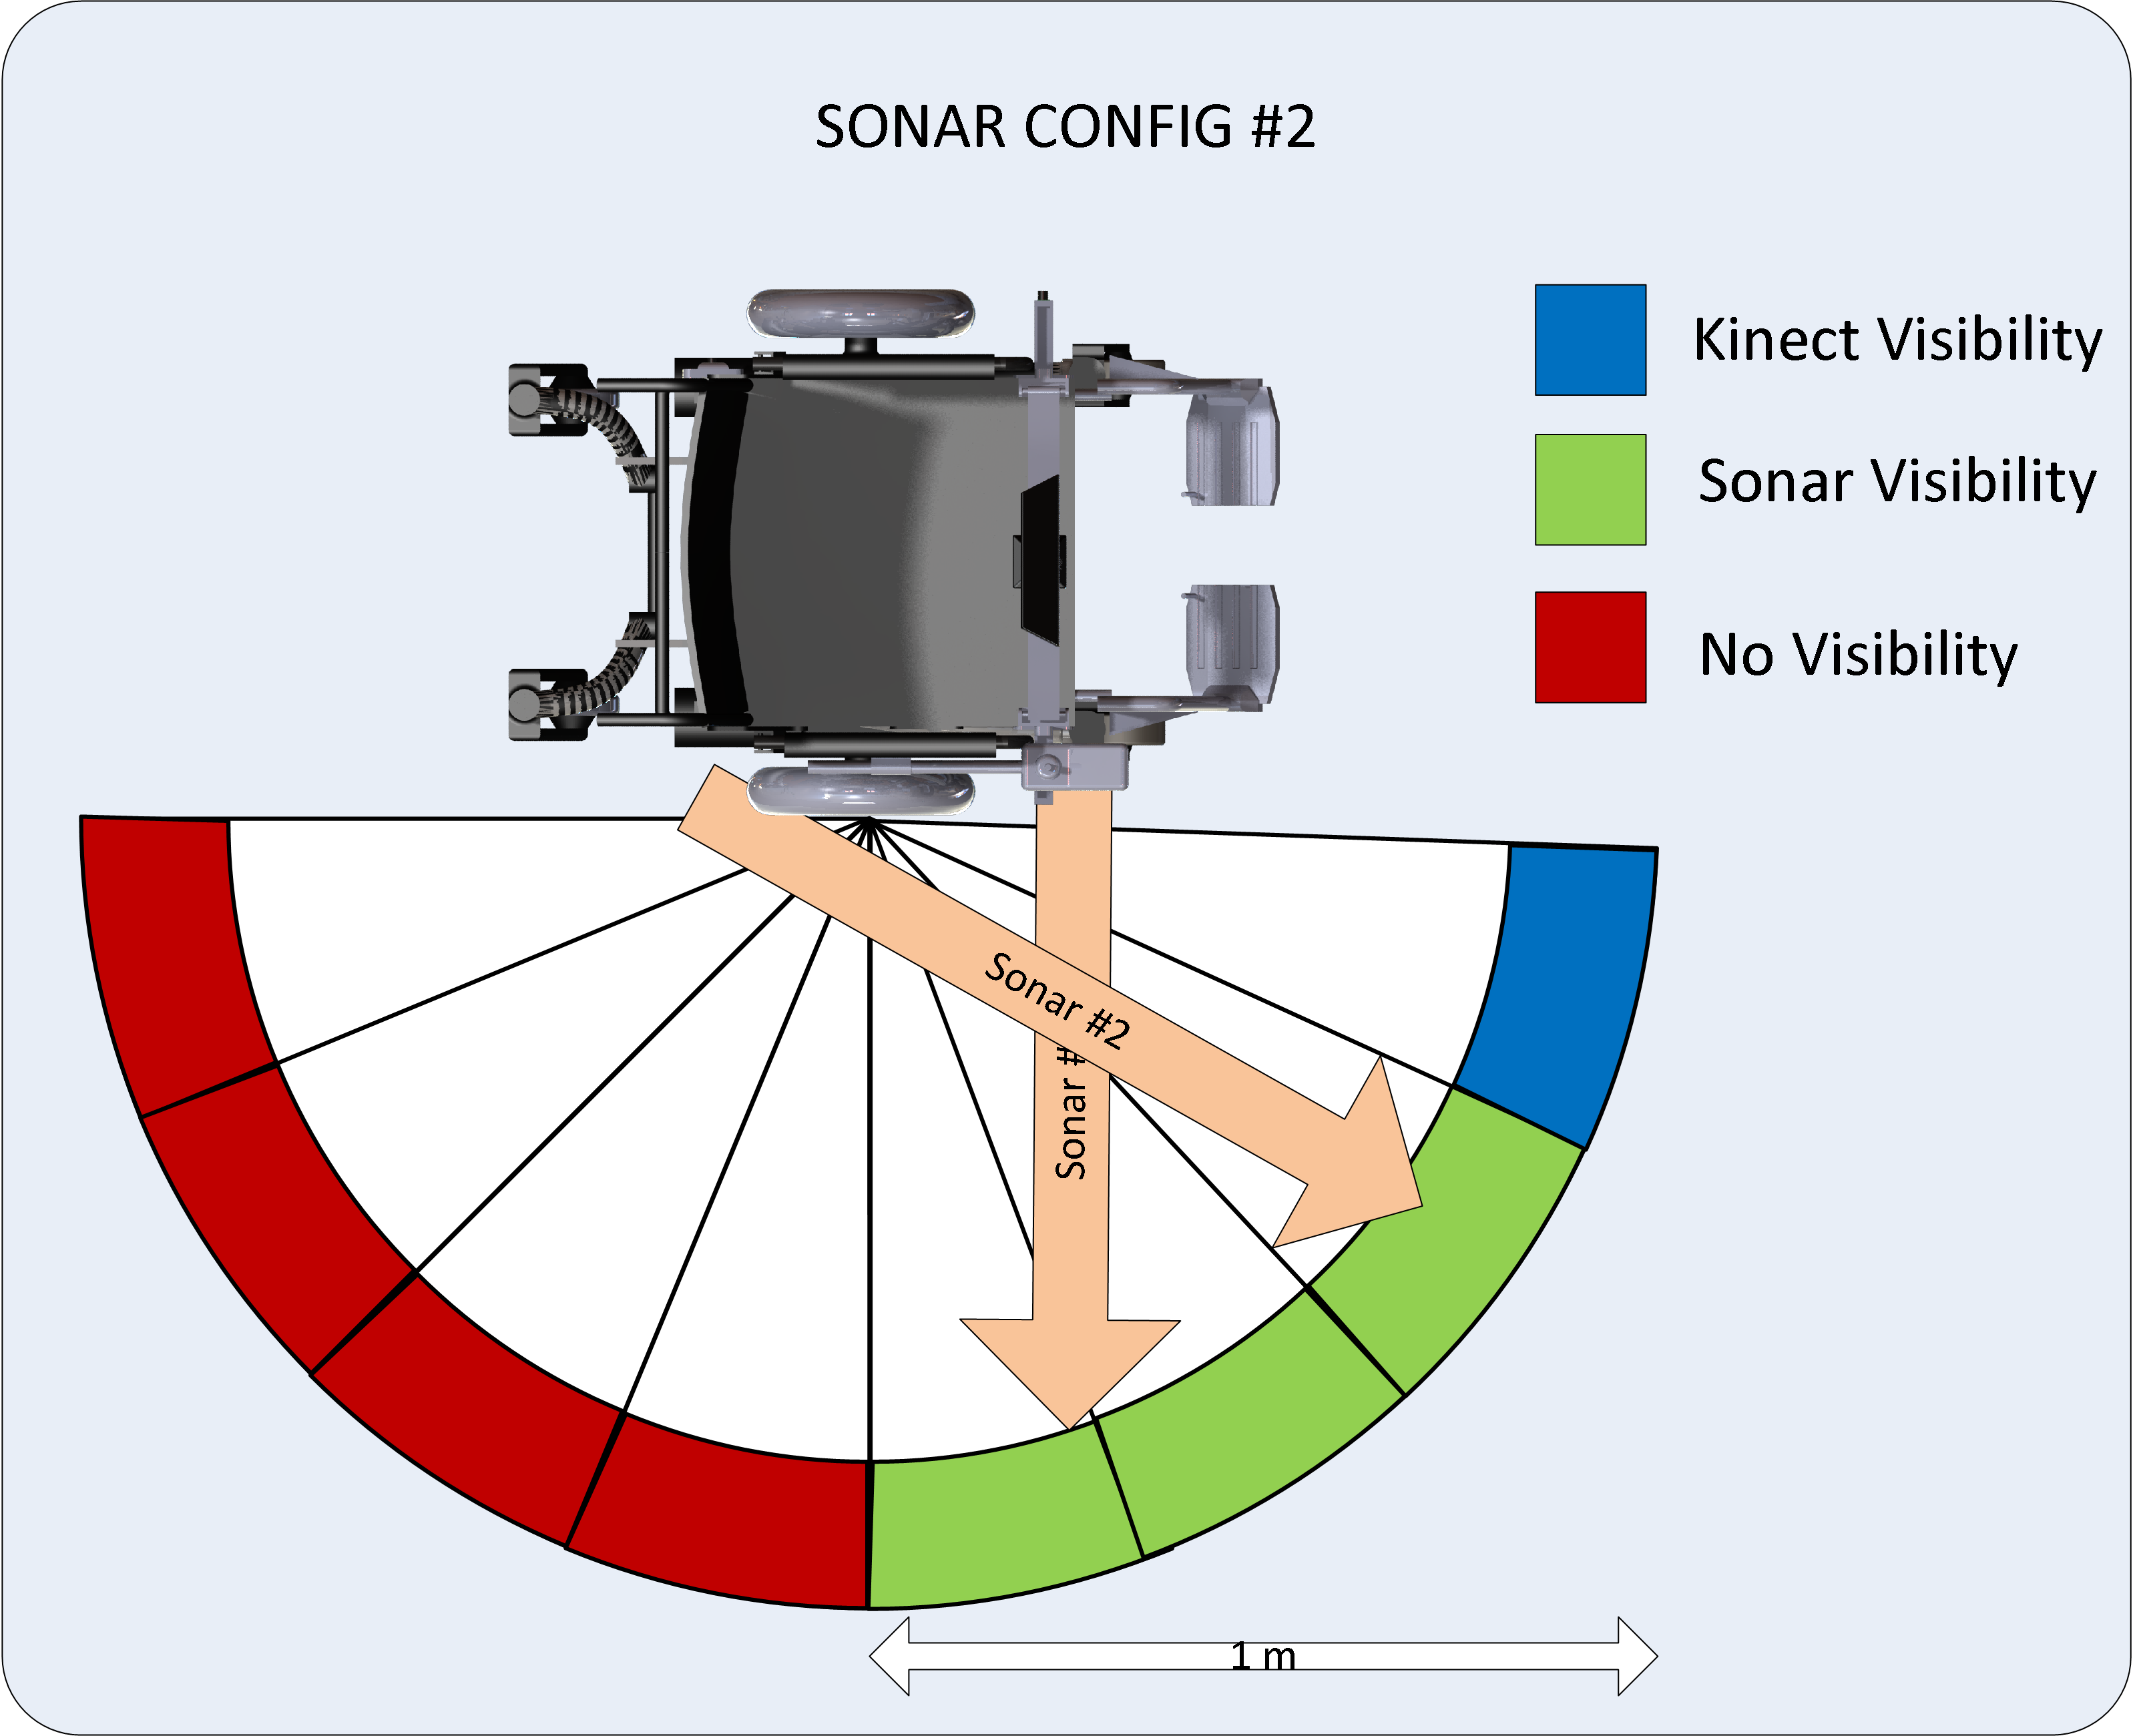
\includegraphics[scale=0.6]{SONAR_Config2.png}
 \caption{SONAR test configuration 2.}
 \label{sonar_2}
\end{figure}

\begin{figure}[hbt]
 \centering
 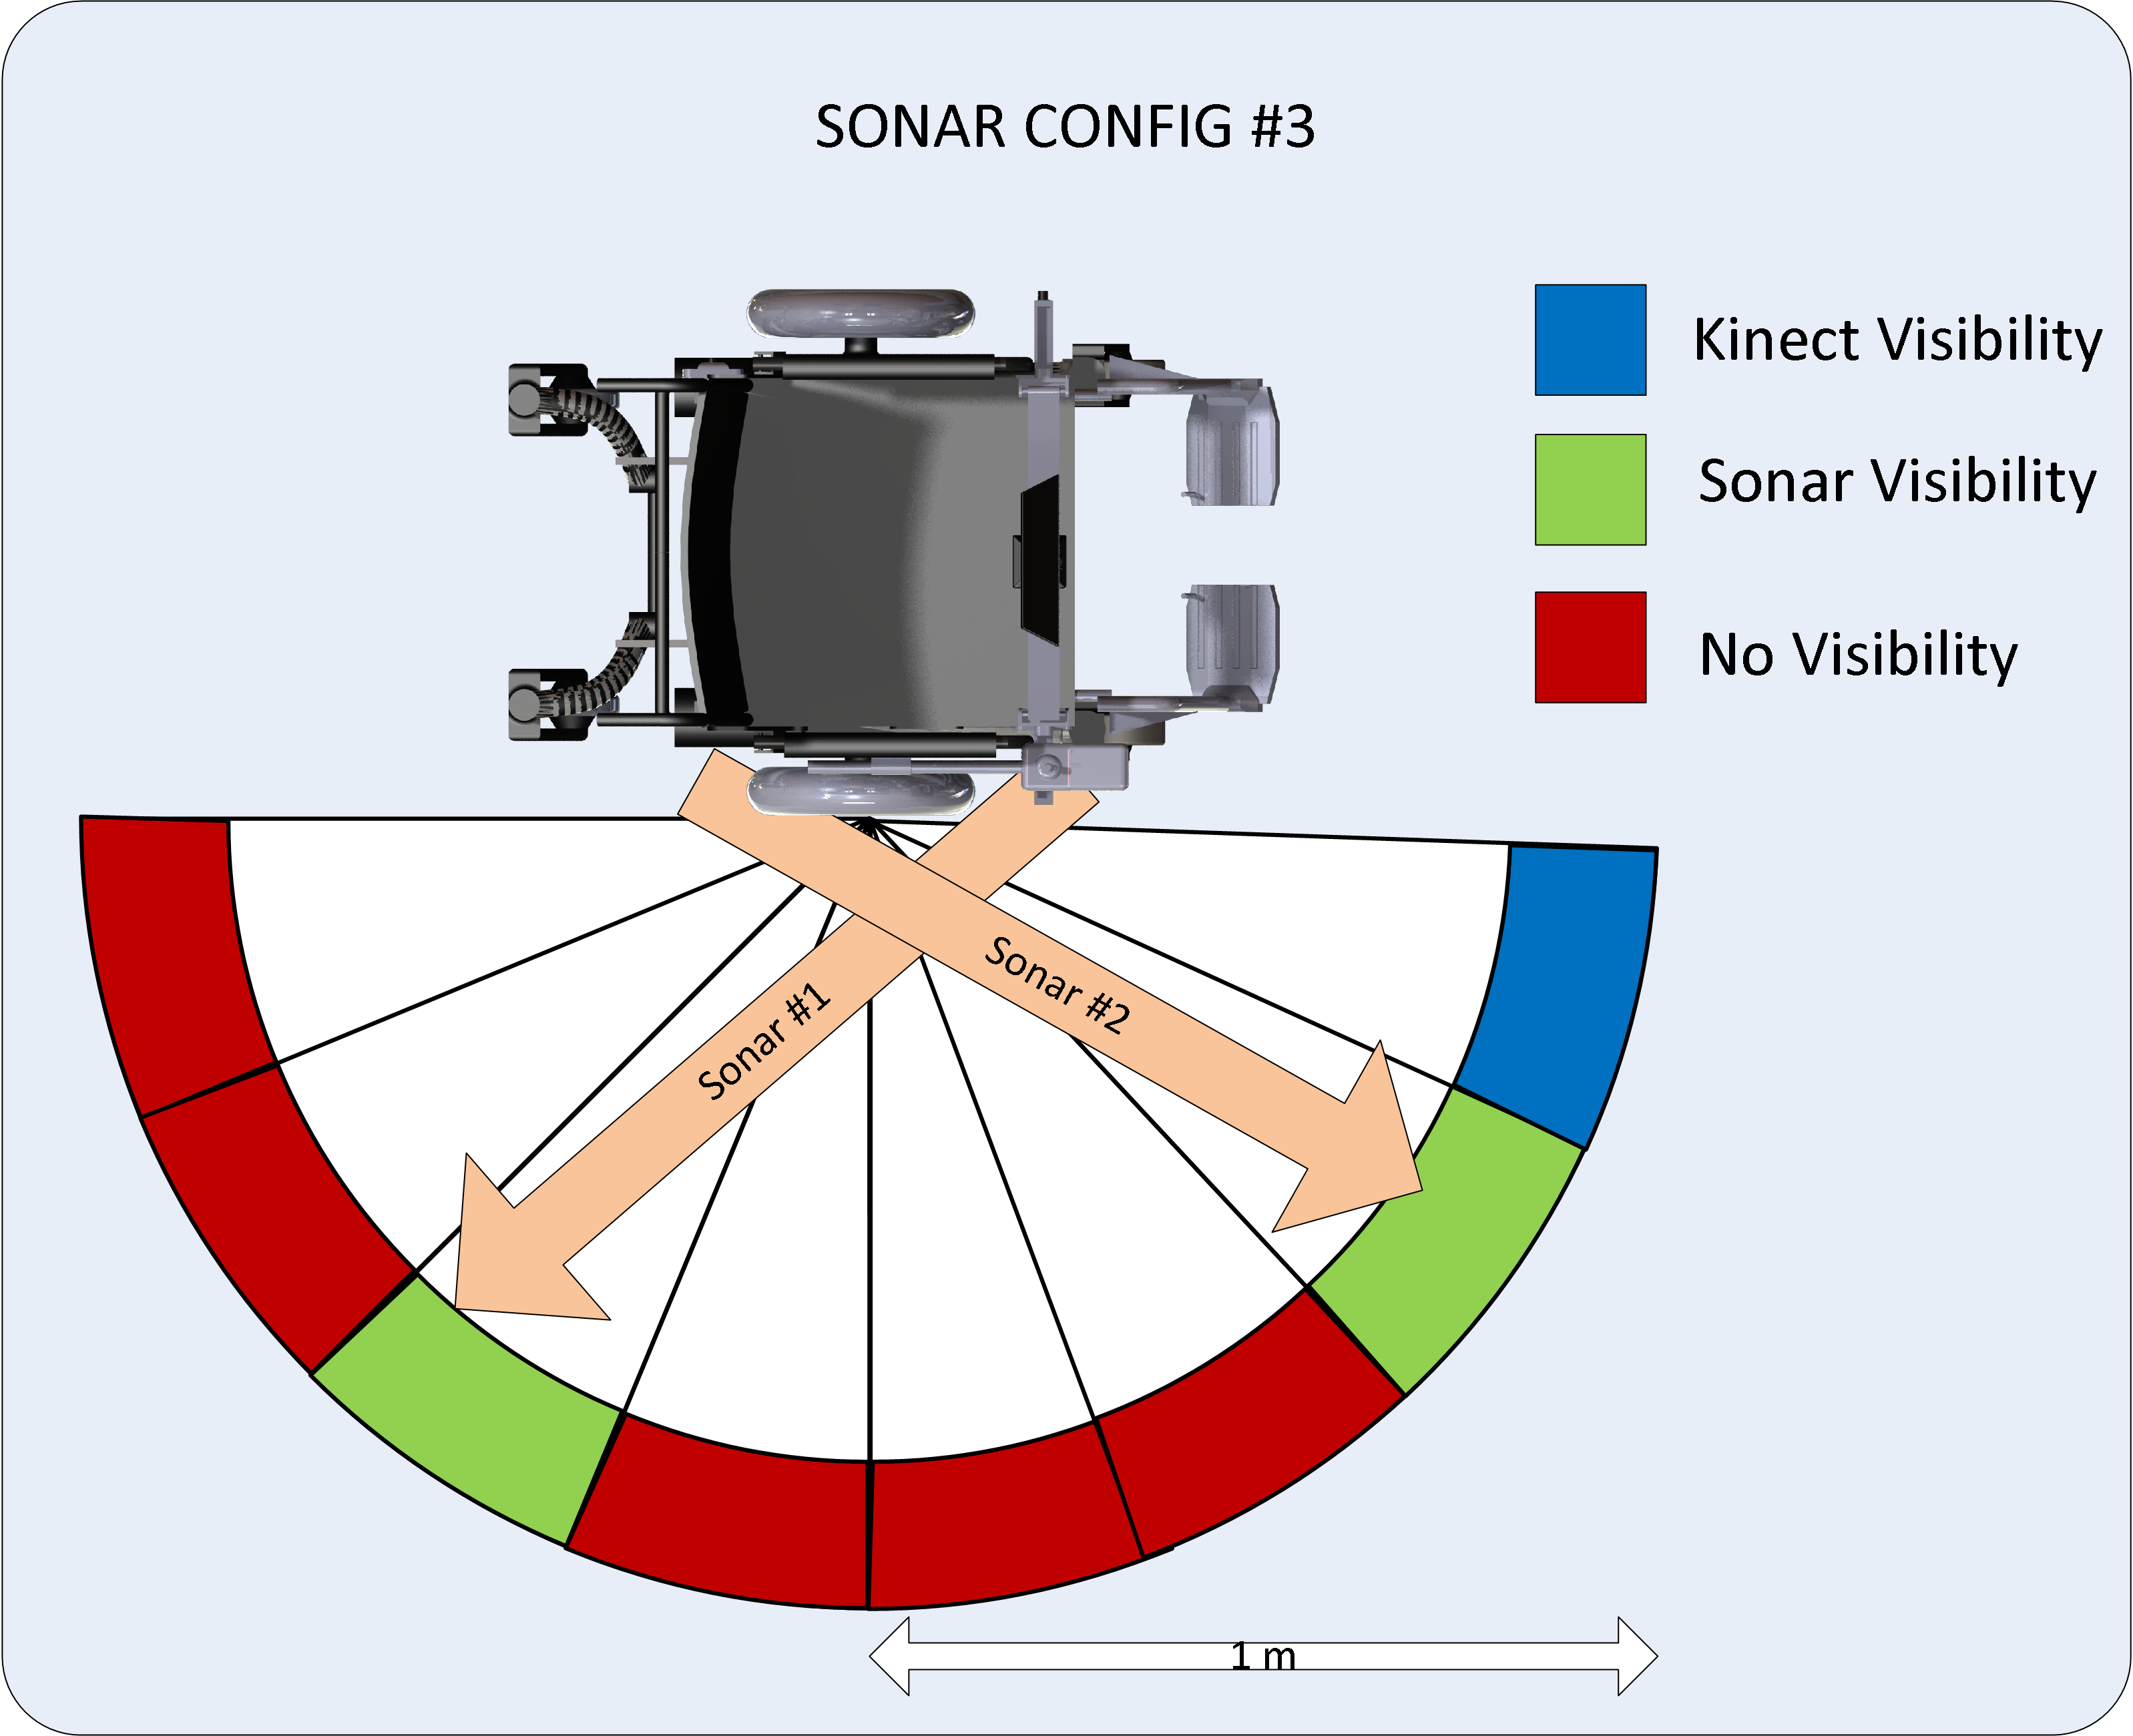
\includegraphics[scale=0.6]{SONAR_Config3.png}
 \caption{SONAR test configuration 3.}
 \label{sonar_3}
\end{figure}

Considering the poor coverage provided by the narrow-beam LV-EZ4 sensors, it is recommended that wider range sensors be used.  For cylindrical objects, the EZ0 model of the same series is sensitive within a cone of approximately $60^\circ$ \cite{lv-ez0}.  Note that, although region of sensitivity depends on object shape, observations indicate that humans are well approximated by large cylindrical dowels.  

With the LV-EZ0 sensors, it is expected that it will be possible to achieve good lateral visibility. Figure \ref{sonar_final} shows the coverage we expect with these sensors.

\begin{figure}[hbt]
 \centering
 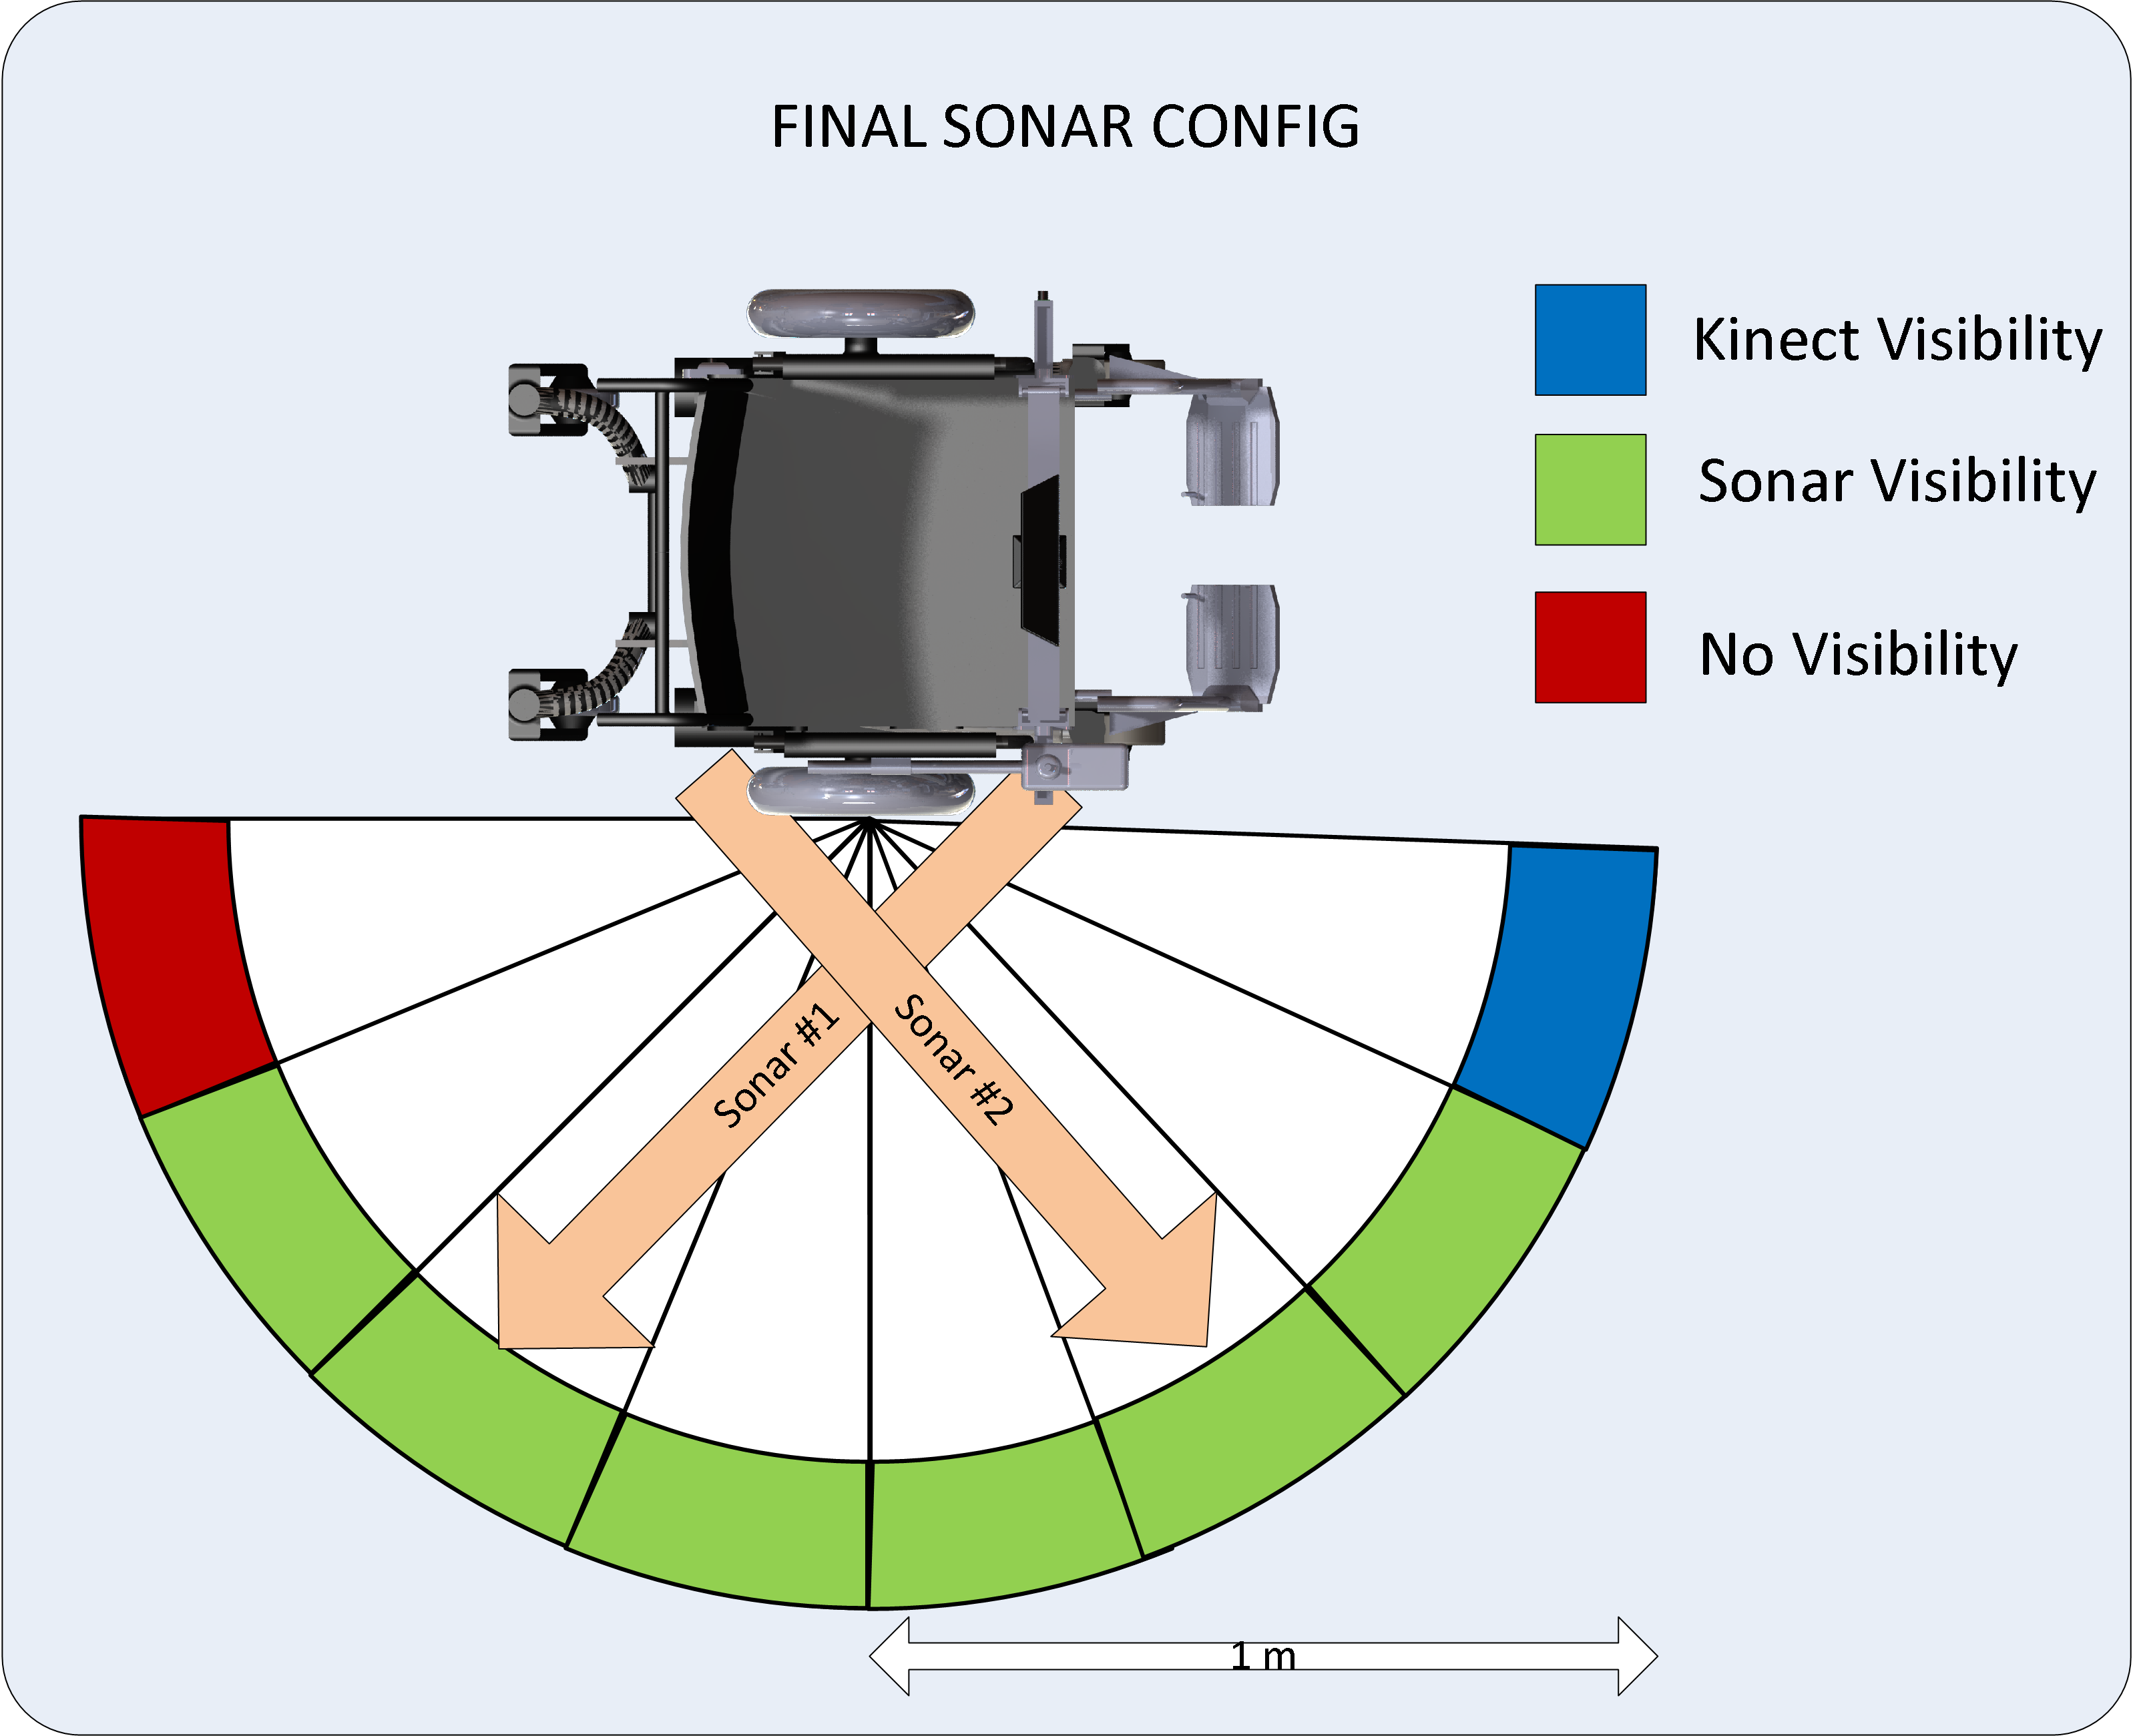
\includegraphics[scale=0.6]{SONAR_Config_Final.png}
 \caption{Final SONAR configuration.}
 \label{sonar_final}
\end{figure}


\section{Systems Integration}
The collision and avoidance software and hardware will need to be integrated with the existing wheelchair for the prototype.

In general, each wheelchair comes from a different manufacturer and could use a different set of joystick, motor controller, and motor. In practice, there seems to be a small number of companies that provide joystick/motor controller combinations to many wheelchair manufacturers, such as Dynamic Controllers.

The chair provided for the prototype is an Invacare chair, using the Dynamic Controls SHARK drive system. The motor controller is model \# DK-PMC08. While no information is provided by the manufacturer (as stated by the manufacturer when the authors attempted to contact Dynamic Controls) about the control protocol used between the joystick and the motor controller, previous systems appeared to be based on CAN-bus (Controller Area Network), a protocol often used in automotive and safety-critical applications). It is possible the authors could reverse engineer this protocol and use it to communicate with the motor controller for purposes of the symposium prototype model.

The joystick itself is coupled inductively to the control board (the control board is housed inside the joystick module, and sends controls over a serial link to the motor controller). A signal excites a coil on the end of the joystick, and this signal is coupled onto four inductors on the control PCB (front/rear/left/right directions) that will change with the joystick's orientation. Only two are strictly required, but four are used for redundancy to eliminate chair movement in the case of a signal fault. Some support is being provided by the manufacturer, Dynamic Controls, to pursue the option of integrating the collision avoidance system by emulating the analog signals seen by the control PCB by the joystick.

A third integration option is to simply replace the Dynamic Controls motor controller with off-the-shelf motor controllers at a fairly low price. This will add some cost to the user if their motor controllers must be replaced when they install a collision-avoidance system, but it is possible this option could be used purely for a prototype with the expectation that the final design would be more integrated with a common wheelchair motor controller.

These three options are being investigated, and the method used to integrate with the prototype unit will be finalized by January of 2012.

\section{Hardware Design}
\begin{figure}[hbt]
 \centering
 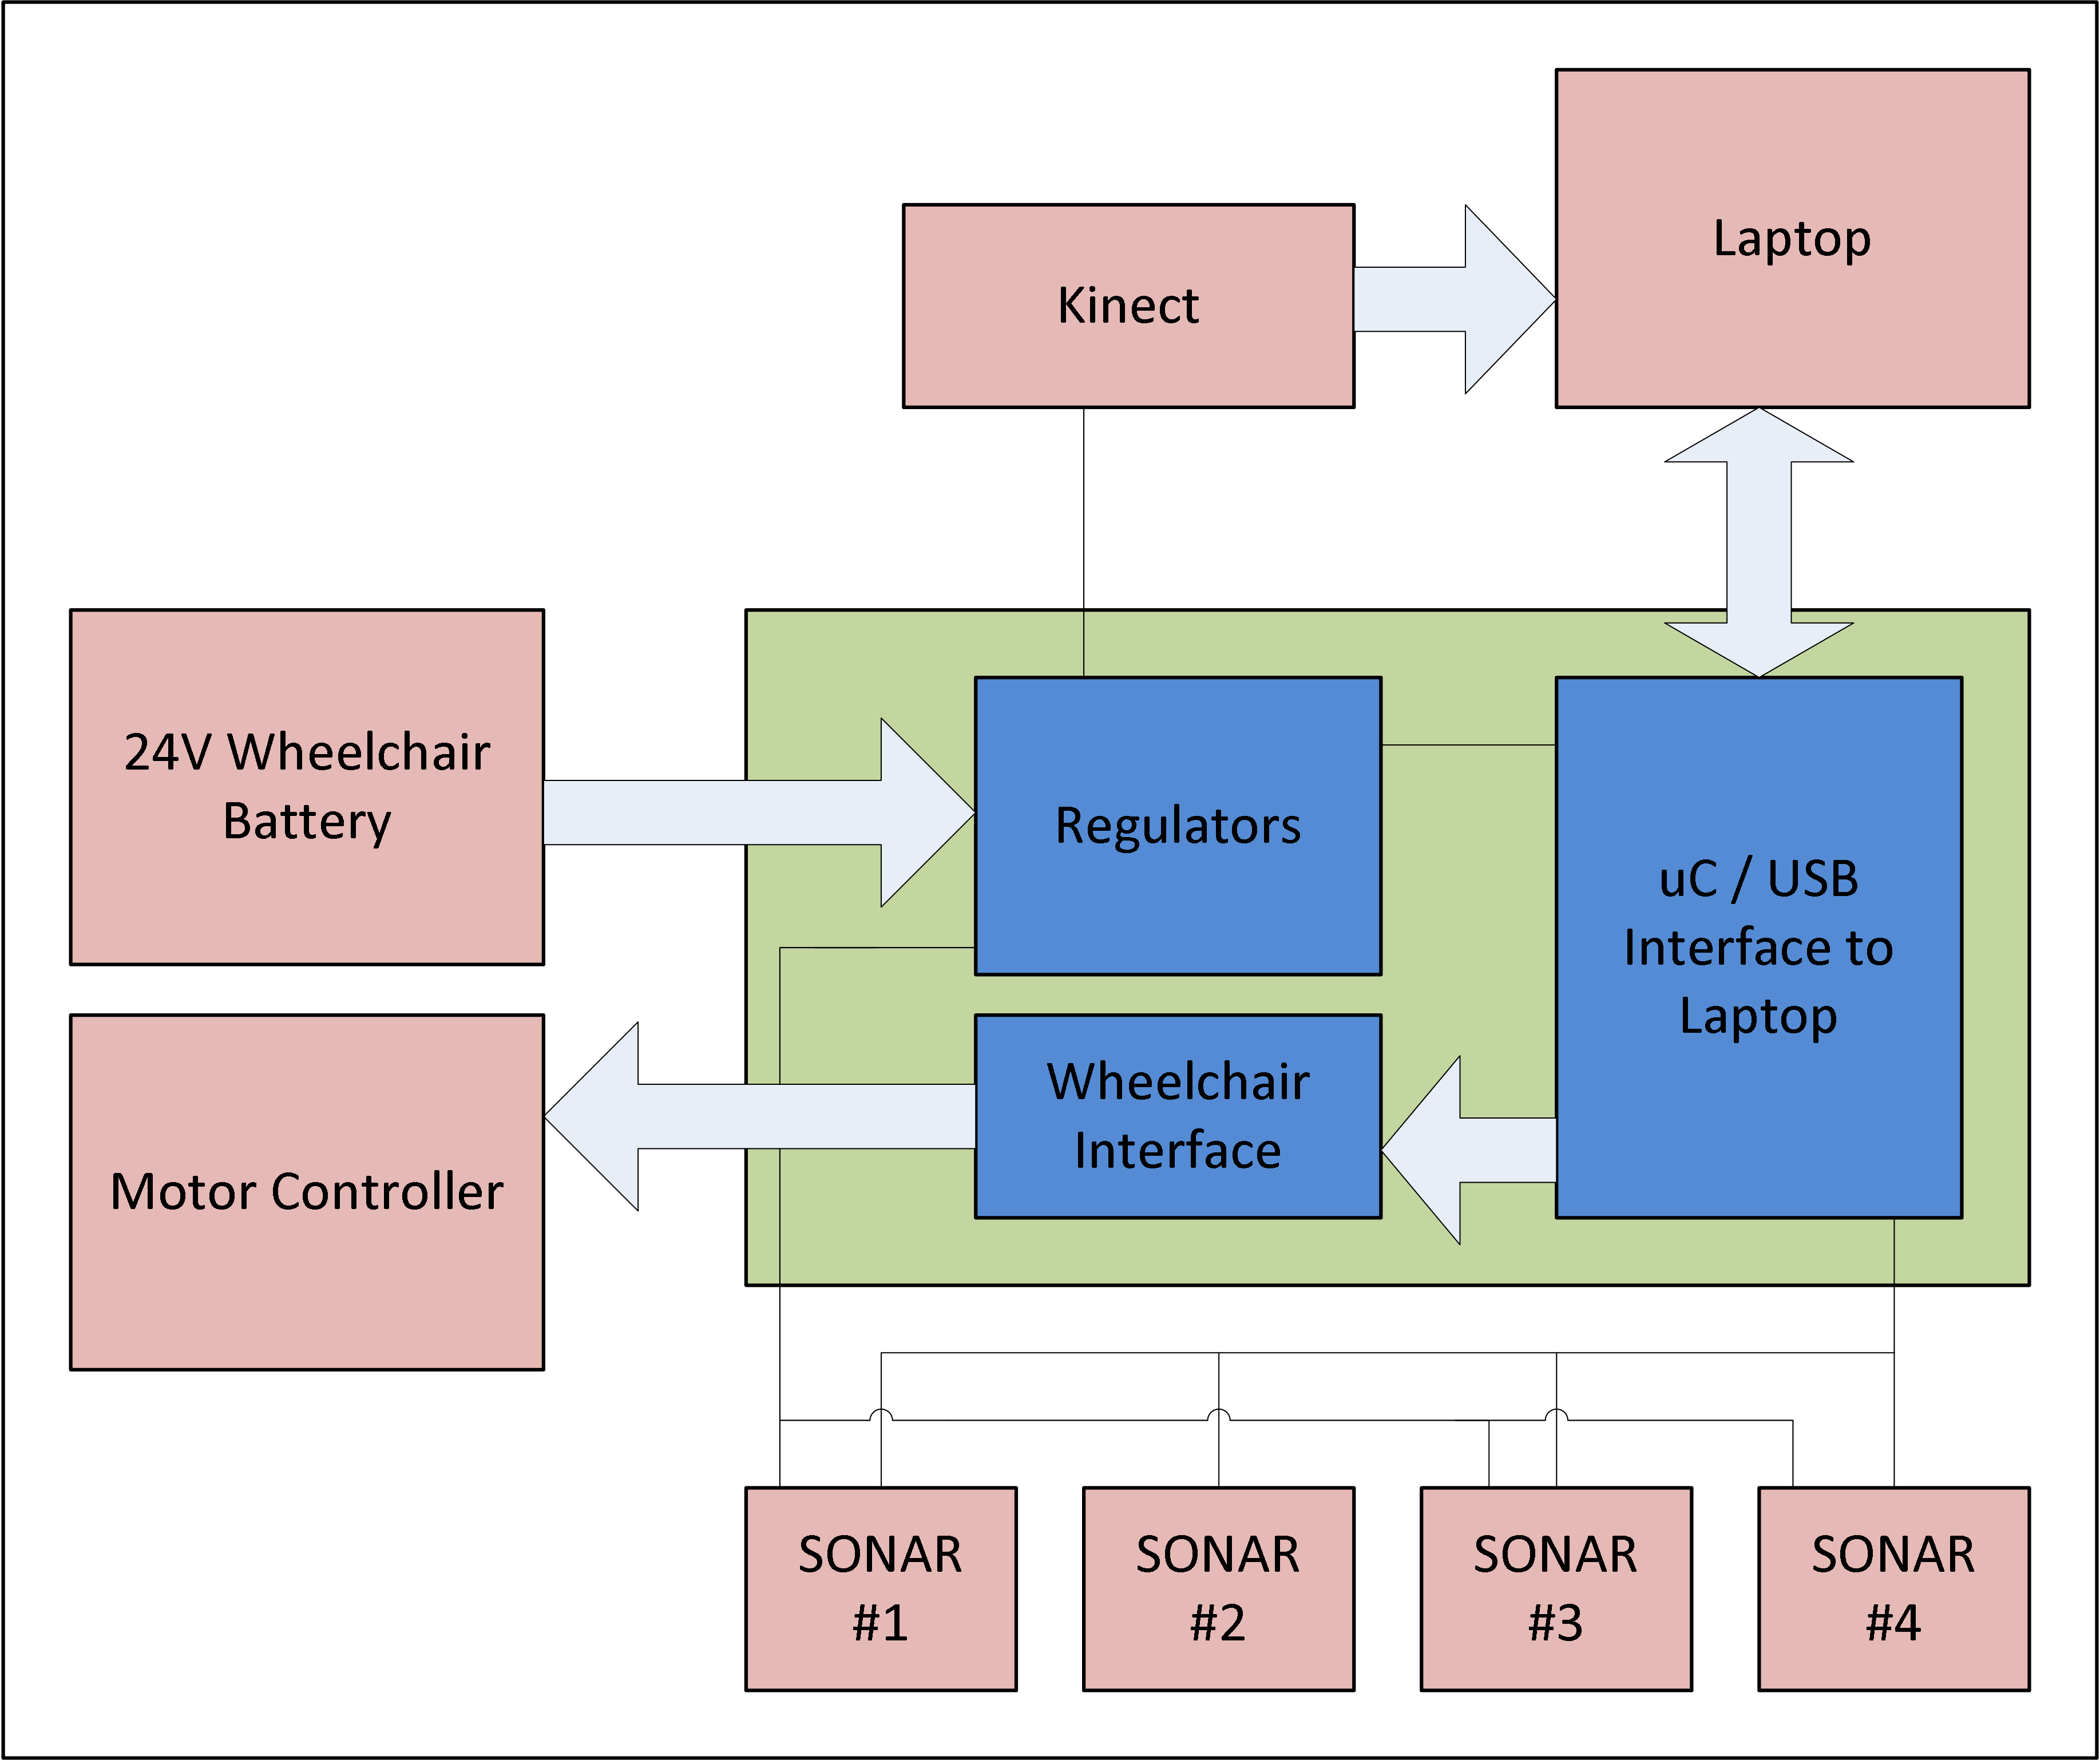
\includegraphics[scale=0.9]{Hardware_Diagram}
 \caption{Hardware Design}\label{fig:hardware}
\end{figure}

In order to interface the software with both the wheelchair and the set of sensors used, a small custom PCB will need to be manufactured. This PCB will have three main functions, as shown in Figure \ref{fig:hardware}.

\subsection{Regulators}
A wheelchair is typically powered off two (sealed or gel) lead acid batteries, for a typical supply voltage of 24-30 Volts. From this voltage a 12 V, 1 Amp supply is required for the Kinect sensor \cite{kinect_power}, and an additional supply of 5 V is required for the sonar sensors and microcontroller on board the PCB.

To perform this task two buck regulators will be used, similar to a sample design shown in Figure \ref{fig:webbench} for a 12 V rail. This design was completed using Webbench Power Architect from National Semiconductor, and allows the easy selection of a regulator to produce a desired output voltage with a given current rating. A similar design will also be completed for a 5 V rail, and then the components fine-tuned and integrated into the PCB.

\begin{figure}[hbt]
 \centering
 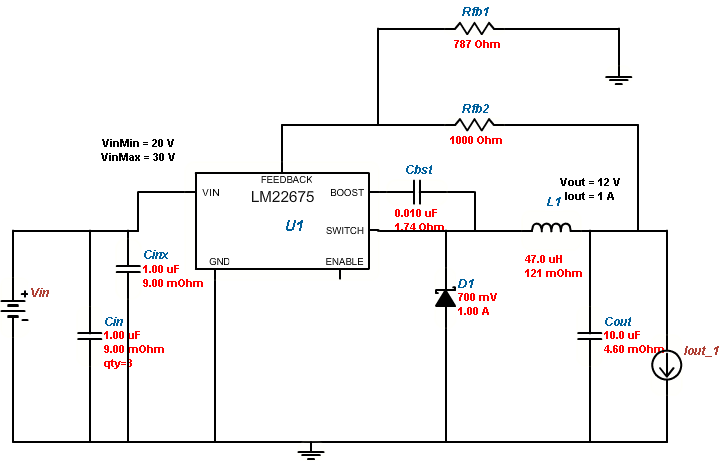
\includegraphics[scale=0.5]{Power_Supply}
 \caption{Power Supply Design for 12 V Rail}\label{fig:webbench}
\end{figure}

\subsection{Wheelchair Interface}
The wheelchair interface will data from a microcontroller on the board, and set the operation of the motor controllers accordingly. The board will not determine the best output for the motors based on the collision map data, this will be done in the software, and the laptop will simply tell this value to the microcontroller on the PCB to be relayed to the motor controller. This section will be finalized based on the interface required for the motor controllers used, and might consist of a serial link via  CAN-bus or a similar protocol, or analog voltage interface (0-5 Volts or similar).

\subsection{USB Interface to Laptop}
A microcontroller will be used to establish a bi-directional USB link to the laptop. The microcontroller will aggregate range information from the sonar sensors, either read in as an analog signal using an analog-to-digital converter or via a RS-232 serial link (depending on sensor model used), and forward this on to the laptop and control software. The microcontroller will then receive commands to be relayed to be relayed to the motor controller, which will be accomplish via the circuitry in the wheelchair interface section shown in Figure \ref{fig:hardware}.

A good choice for microcontroller to be used would be the MSP 430 by Texas Instruments. A sample circuit including bi-directional USB interfacing is shown in an Application Note by TI \cite{MSP430_USB}, and the authors have some experience designing hardware using this microcontroller.

\section{Software Design}
\begin{figure}[hbt]
 \centering
 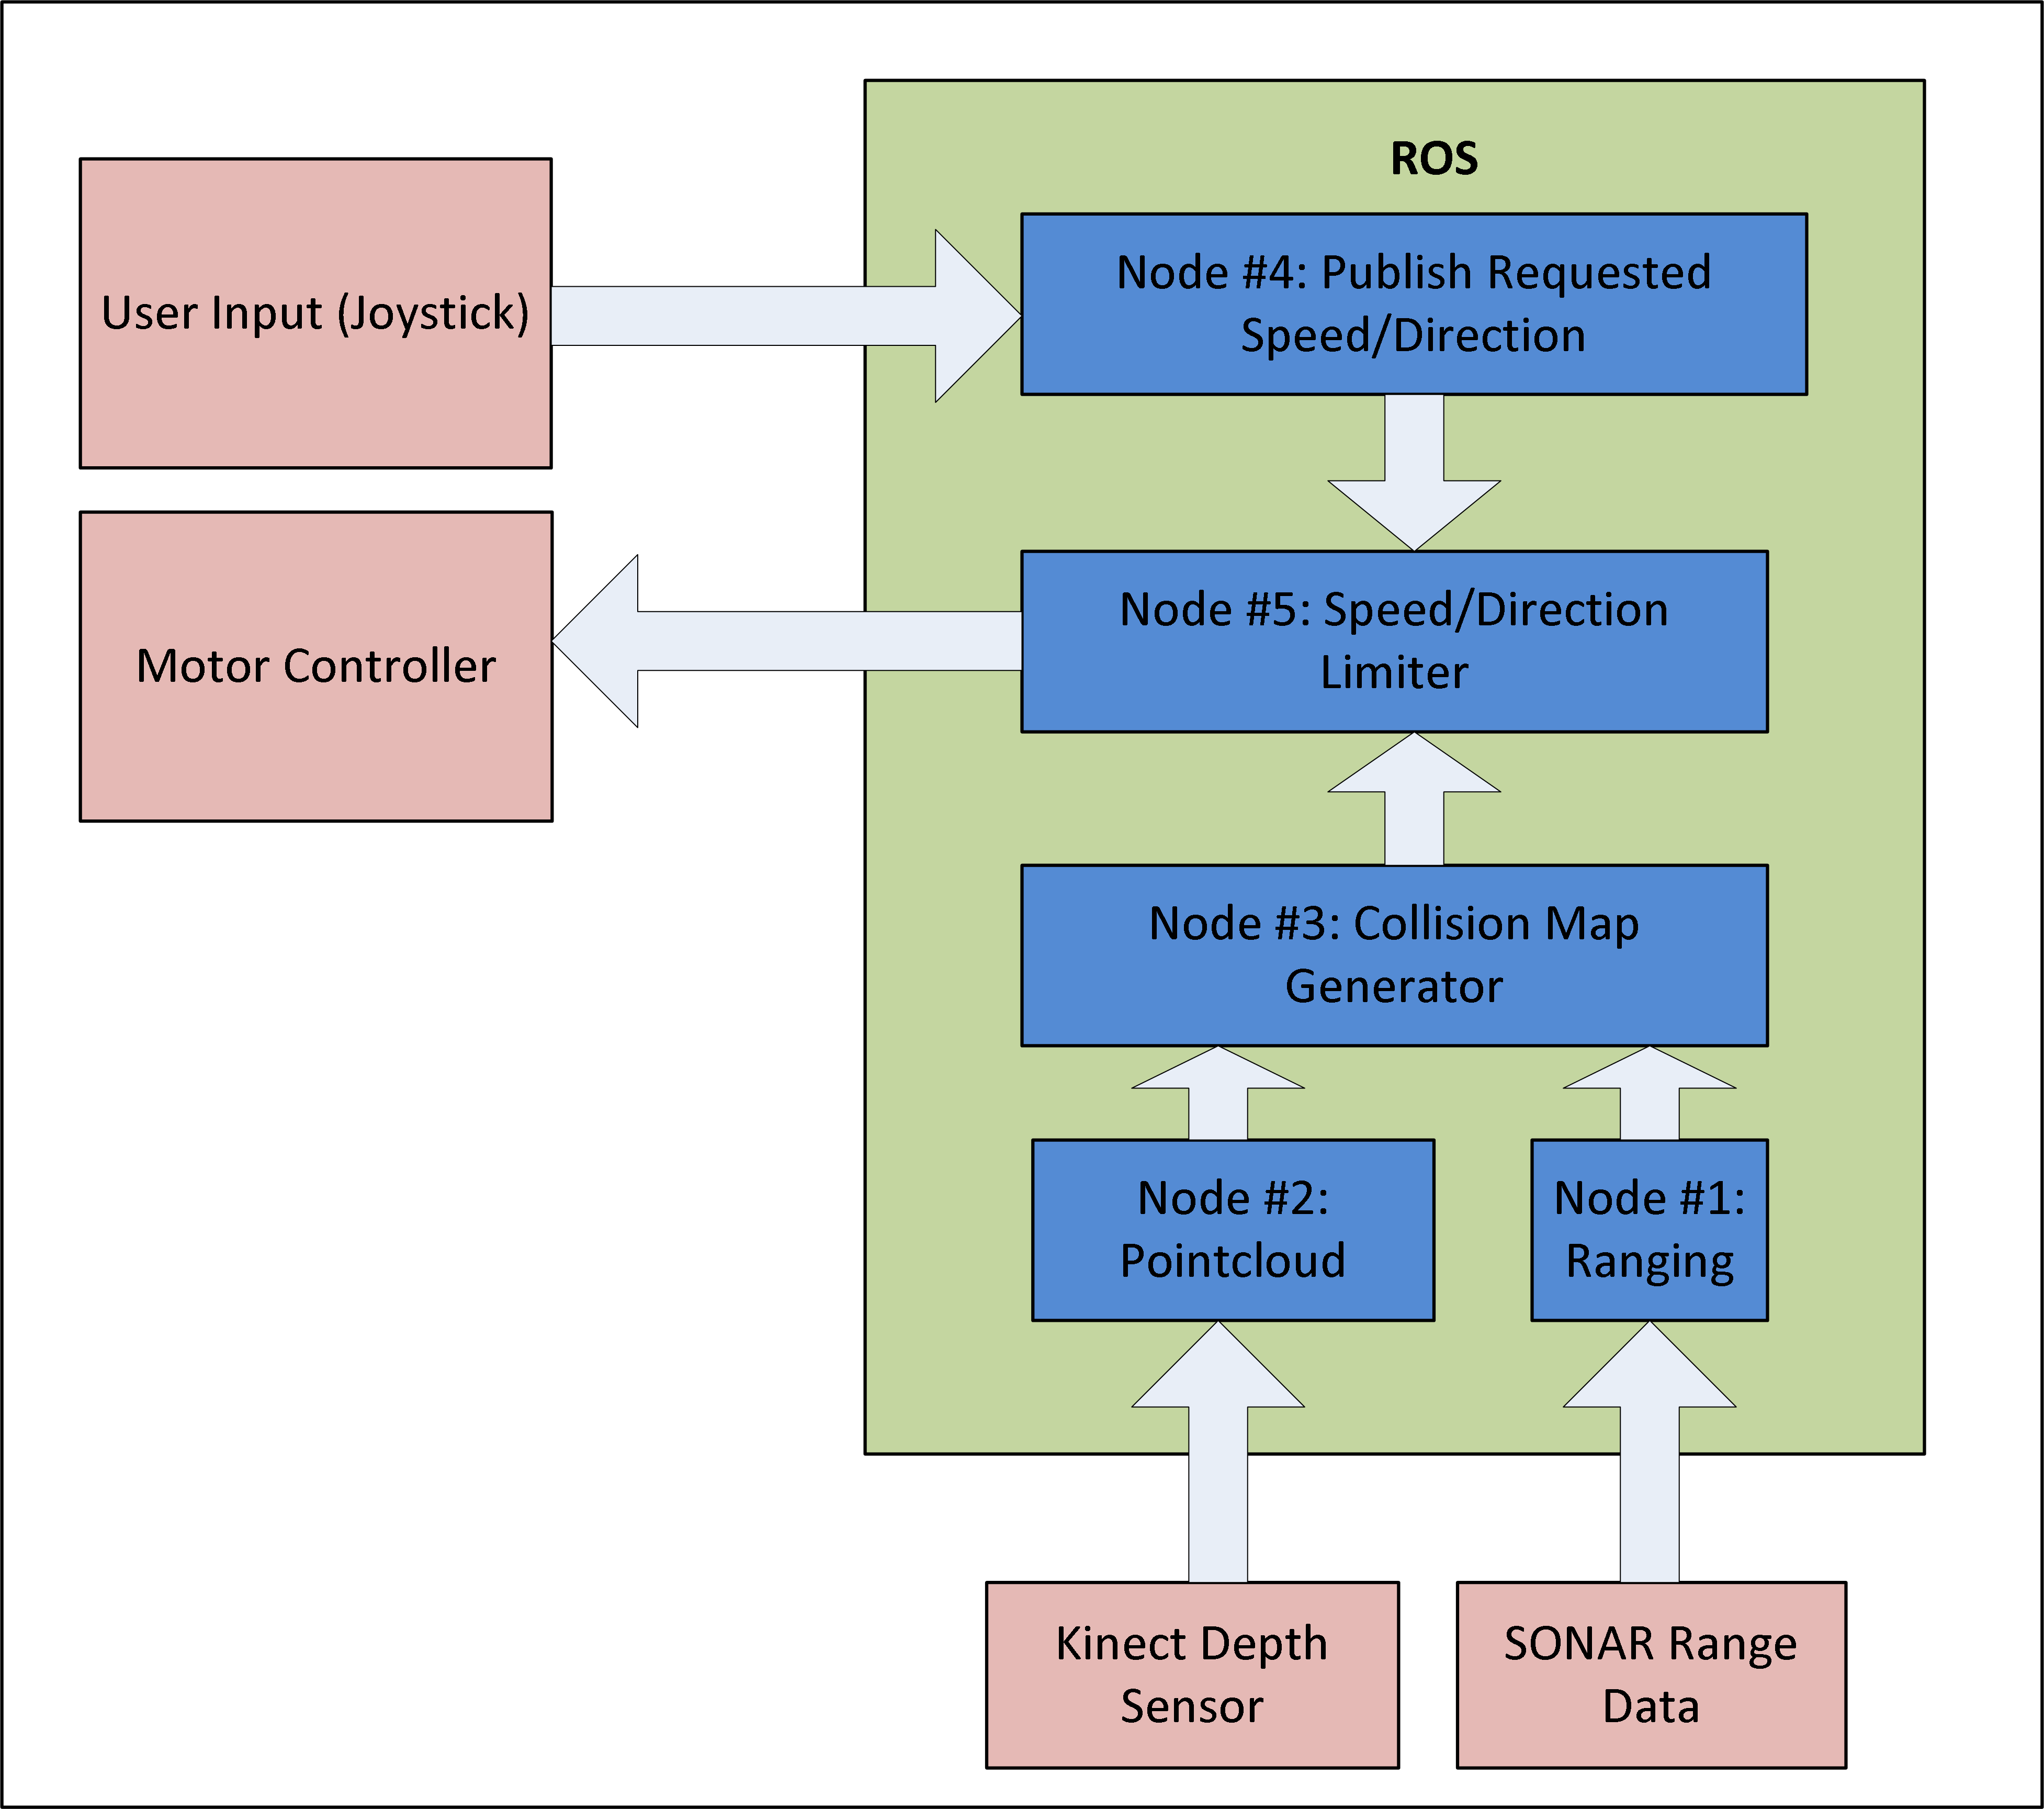
\includegraphics[scale=0.9]{Software_Diagram}
 \caption{Software Design}\label{fig:software}
\end{figure}

Figure \ref{fig:software} shows an overview of the intended software architecture.  Software will be built on the Robot Operating System (ROS) \cite{ROS}, which is a distributed message passing system capable of running on Linux systems.  ROS systems are organized into a network of simple nodes, which co-operate to produce complex aggregate behaviour. 

\subsubsection{Node 1: Ranging}
The ranging node is responsible with communicating with the micro-controller in order to obtain range data from the ultrasonic rangefinders.  It publishes parsed range data.

\subsubsection{Node 2: Point Cloud}
The point cloud node communicates with the Kinect, in order to obtain depth map data.  It publishes point cloud data.

\subsubsection{Node 3: Collision Map Generator}
The collision map generator node is responsible for interpreting poinrt cloud and rangefinder data.  These data are projected into a 2-D occupancy grid in the vehicle frame.  In the simplest case, collision map generation is stateless, and ignores previous data in the interpretation of new sensor data.  If this does not provide sufficient accuracy, the collision map generator might also use state estimates to project old information forward, improving estimates.  

This node subscribes to point cloud and rangefinder data, and publishes collision maps.

\subsubsection{Node 4: Joystick}
The joystick node is responsible for communicating with the joystick, in order to obtain speed and direction commands from the user.  It publishes joystick state.

\subsubsection{Node 5: Speed / Direction Limiter}
The speed / direction limiter node is responsible for communicating with the motor controller in order to set wheel velocities.  It uses a collision map and a wheelchair motion model to assess whether a particular command is likely to lead to a collision.  If necessary, it adjusts user commands in order to avert collisions.

This node subscribes to collision map and joystick command data.  It does not publish anything.

\chapter{Schedule and Budget}

\section{Schedule}
\begin{figure}[htb]
 \centering
 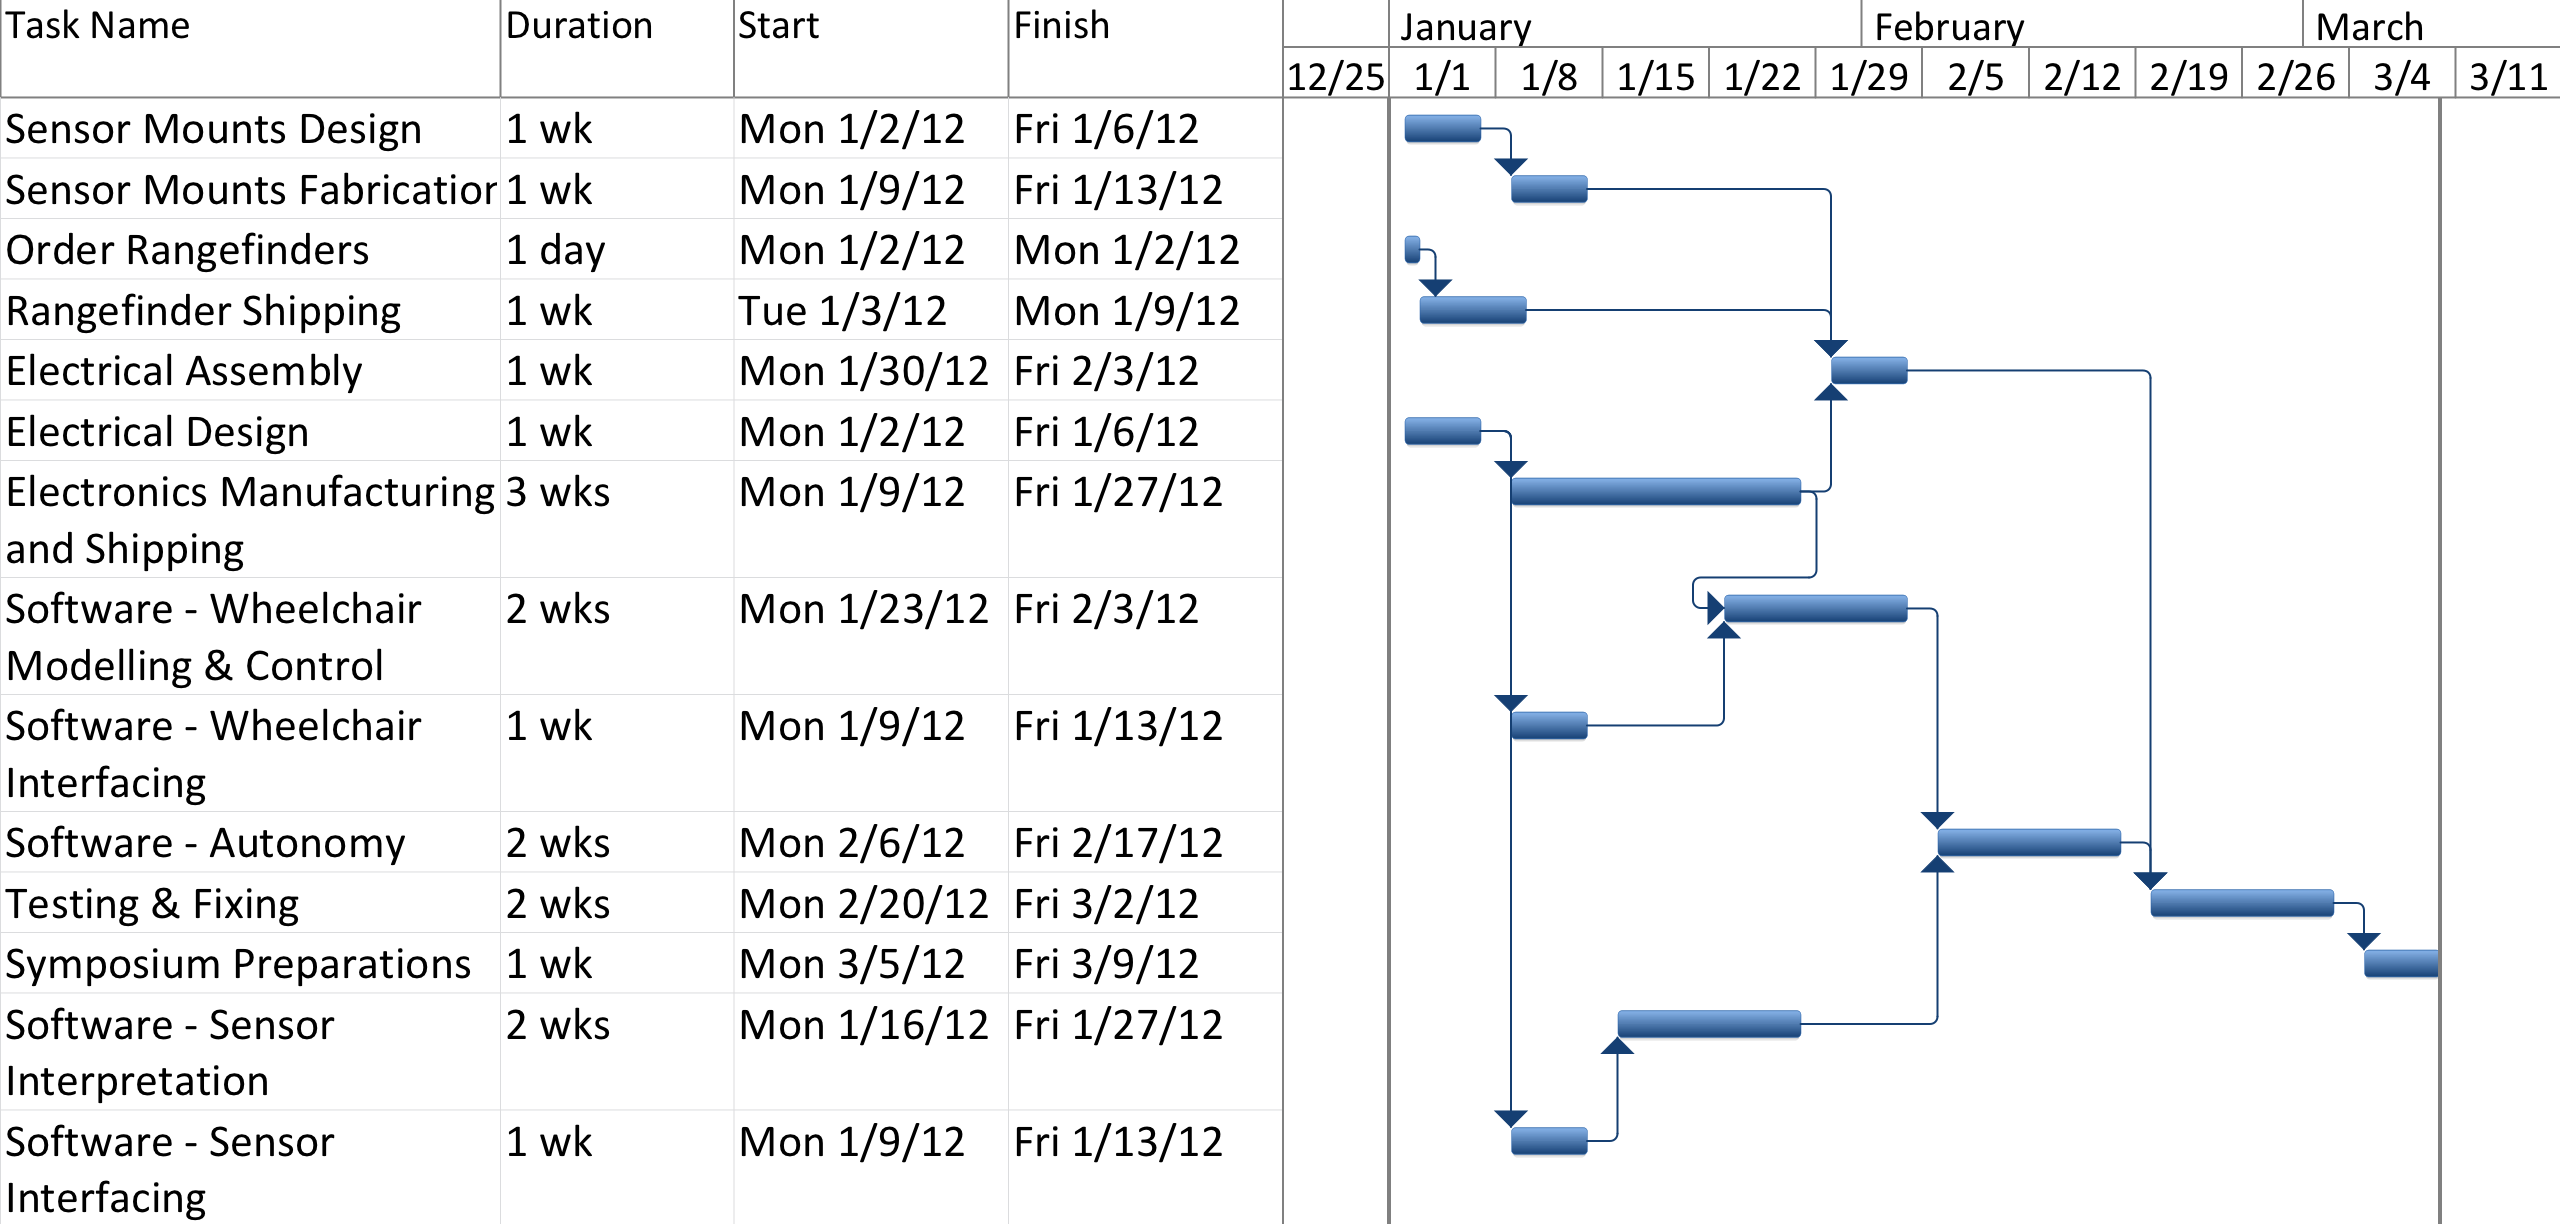
\includegraphics[scale=0.6]{gantt.png}
 \caption{Production schedule for the prototype}
 \label{schedule}
\end{figure}

Figure \ref{schedule} shows the prototype production gantt chart.  It may be seen that the prototype is expected to be completed about a week before the March symposium date.  The timeline is dominated by electrical and software tasks; if possible, it would be especially advantageous to begin electrical design work early.

\section{Bill of Materials}
\vspace{0.5cm}
\begin{figure}[ht]
\centering
\begin{tabular}{|l|c|c|c|}
\hline
Part & Count & Cost (CAD) & Total (CAD) \\
\hline \hline
Xbox Kinect & 1 & 150 & 150 \\
\hline
Xbox Kinect Mount & 1& 15 & 15 \\
Sonar Sensor & 4 & 30 & 120 \\
\hline
Sheet Metal & 1 & 12 & 12 \\
\hline
Spacers & 8 & 0.25 & 2 \\
\hline
PCB \& Components & 1 & 150 & 150 \\
\hline
Basic Netbook & 1 & 250 & 350 \\
\hline
\hline
Total&&&789\\
\hline
\end{tabular}
\caption{Bill of Materials}
\label{tab:BOM}
\end{figure}

Note that figure \ref{tab:BOM} shows the expected cost for the prototype system.  It is expected that, in production, economies of scale will reduce the unit cost to below the target price of \$500.

\chapter{Conclusion}

The design of a collision avoidance system for a powered wheelchair is discussed.

It has been decided that a combination of the Microsoft Kinect and wide-angle ultrasonic rangefinders will satisfy sensing requirements.  Several possible sensor mount designs are presented, and a final decision is made.  Software architecture is discussed at a high level.

The prototype is expected to be completed in time for symposium, and it is expected to meet requirements.

\chapter*{Appendix A} \label{mech_drawings}
\addcontentsline{toc}{chapter}{Appendix A - Mechanical Drawings}
\begin{figure}[hbt]
 \centering
 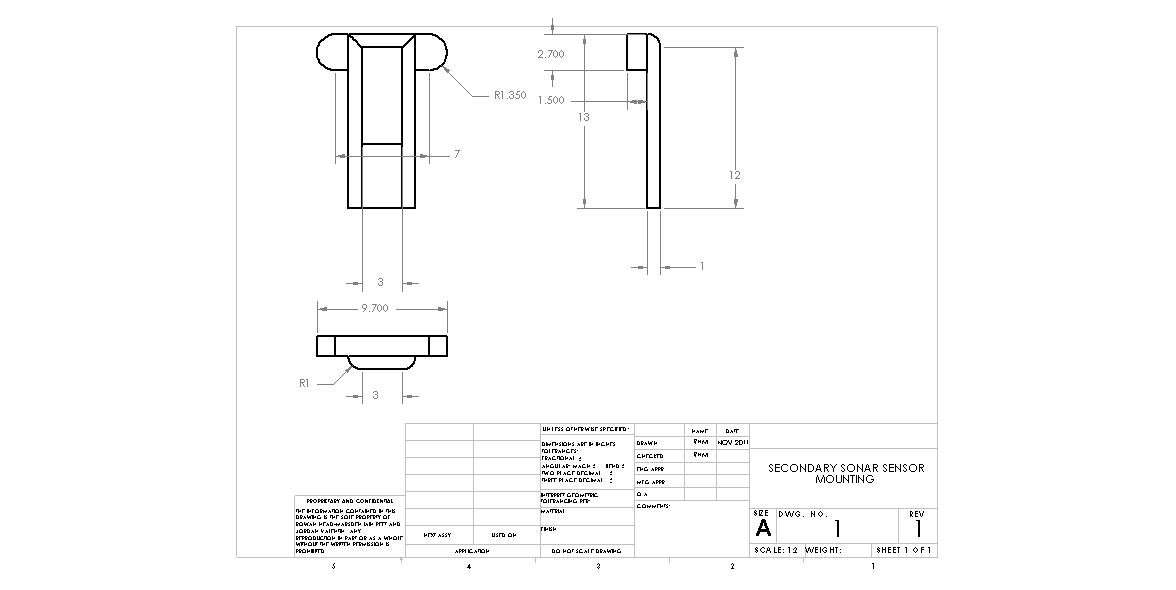
\includegraphics[scale=0.65]{Drawing_Left}
 \caption{Secondary Sonar Sensor Mounting}
\end{figure}

\begin{figure}[hbt]
 \centering
 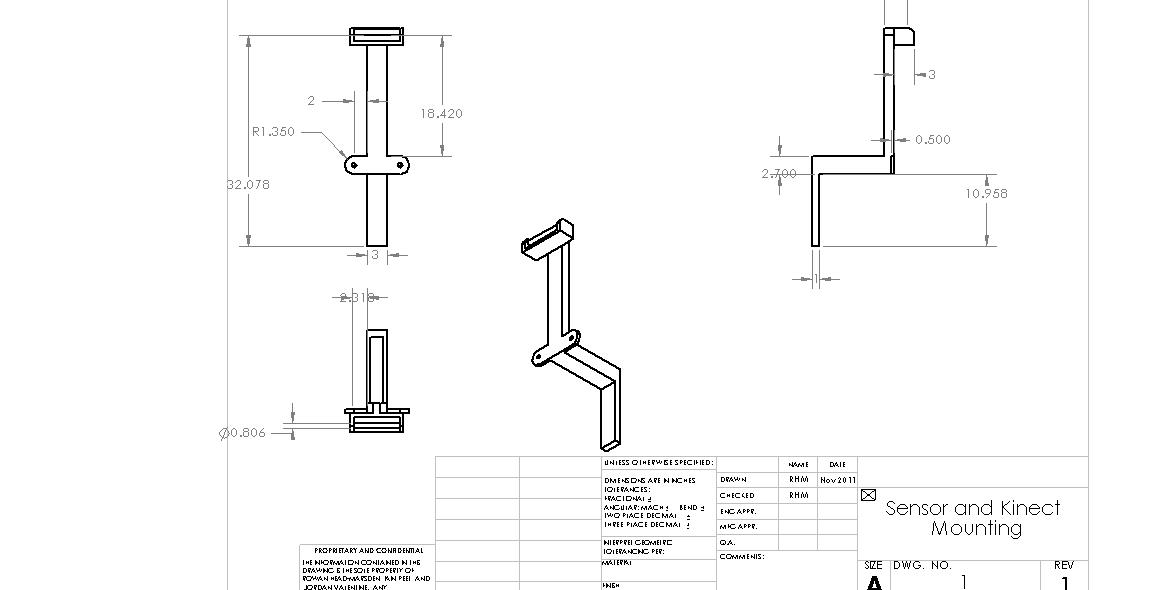
\includegraphics[scale=0.5]{Drawing_Right}
 \caption{Sensor and Kinect Mounting}
\end{figure}

\begin{figure}[hbt]
 \centering
 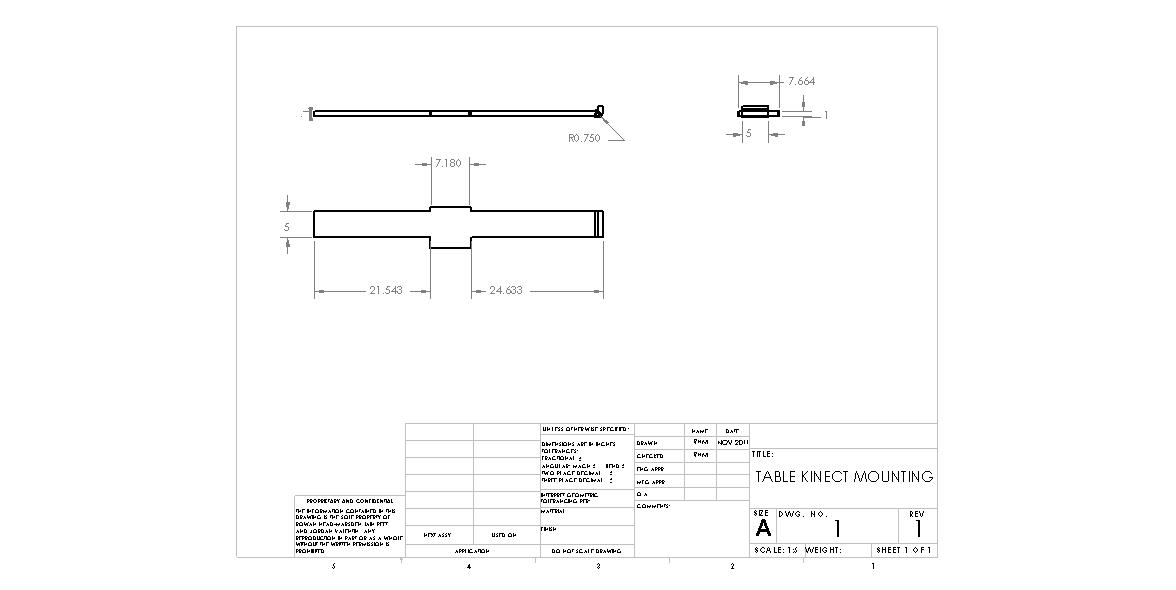
\includegraphics[scale=0.65]{Drawing_Table}
 \caption{Table Kinect Mounting}
\end{figure}


\begin{thebibliography}{9}
 \addcontentsline{toc}{chapter}{Bibliography}

 % NB: cite these with \cite{item}

 \bibitem{patent:computer_controlled}
  L. Fehr, S. Skaar, G. Del Castillo. \\
  \emph{Computer Controlled Power Wheelchair Navigation System.} \\
  U.S. Patent 2008/7383107B2, Jun. 3, 2008.
 \bibitem{patent:power_wheelchair}
  G. Griggs, T. Dutta, G. Fernie. \emph{Powered Wheelchair},\\
  U.S. Patent 2010/0082182A1, Apr. 1, 2010.
 \bibitem{patent:wheelchair_method}
  T. Smithers, U. Urriticoechea, U. Campos. \\
  \emph{Wheelchair and Method for Correcting the Guidance of a Wheelchair.} \\
  U.S. Patent 2011/0130940A1, Jun. 2, 2011.
 \bibitem{NASA}
  NASA. \emph{NASA-STD-3000. Anthropometry and Biomechanics.}\\
  http://msis.jsc.nasa.gov/sections/section03.htm, Jul. 1995.
\bibitem{primesense}
  \emph{Our Full 3D Sensing Solution}, \\
  \mbox{http://www.primesense.com/en/technology/115-the-primesense-3d-sensing-solution} \\
  2011.
 \bibitem{OpenNI}
  http://www.openni.org/
 \bibitem{ROS}
  http://www.ros.org/
 \bibitem{point_clouds}
  http://pointclouds.org/
 \bibitem{wheelchair_data}
  Invacare. \emph{Nutron R51LXP. Invacare Product Catalogue.} \\
  http://www.invacare.ca/cgi-bin/imhqprd/inv\_catalog/prod\_cat\_detail.jsp?s=0\&prodID=R51LXP\\
 Jan. 2011.
\bibitem{kinect_prec}
  L. Yiping. \\
  \emph{openni\_kinect/kinect\_accuracy}, http://www.ros.org/wiki/openni\_kinect/kinect\_accuracy\\
  Jun. 27, 2011.
 \bibitem{lv-ez4}
  MaxBotix Inc, \emph{LV-EZ4 Datasheet},  2011
 \bibitem{lv-ez0}
  MaxBotix Inc, \emph{LV-EZ0 Datasheet},  2011
 \bibitem{kinect_power}
  M. Wise.  \emph{Adding a Kinect to an iRobot Create} \\
  http://www.ros.org/wiki/kinect/Tutorials/Adding\%20a\%20Kinect\%20to\%20an\%20iRobot\%20Create\\
  May 2, 2011.
 \bibitem{MSP430_USB}
  A. Dannenberg. (2006, October). \emph{MSP430 Connectivity Using TUSB3410},\\
  http://www.ti.com/lit/an/slaa276a/slaa276a.pdf
\end{thebibliography}


\end{document}